\documentclass[reqno,12pt,oneside]{report} % right-side equation numbering, 12 point font, print one-sided 
%\documentclass[reqno,12pt,twoside,openright]{report} % right-side equation numbering, 12 point font, print two-sided, Chapters start on odd pages. Rackham only accepts one-sided, so this is for personal printings.

\usepackage{rac}         % Use Rackham thesis style file
\usepackage{aas_macros}  % To allow the reading of ADS journal references in the bibliography
\usepackage[intlimits]{amsmath} % Puts the limits of integrals on top and bottom
\usepackage{amsxtra}     % Use various AMS packages
\usepackage{amsthm}
\usepackage{amssymb}
\usepackage{amsfonts}
\usepackage{graphicx}    % Add some packages for figures. Read epslatex.pdf on ctan.tug.org
\usepackage{rotating}
\usepackage{color}
\usepackage{placeins}
\usepackage{makecell}
\usepackage{epsfig}
% \usepackage{subfigure}   % To make subfigures. Read subfigure.pdf on ctan.tug.org
\usepackage{verbatim}
\usepackage[numbers]{natbib}      % Allows you to use BibTeX
\usepackage[printonlyused]{acronym} % For the List of Abbreviations. Read acronym.pdf on ctan.tug.org
\usepackage{setspace}    % Allows you to specify the line spacing
%\usepackage{mathptmx}
\usepackage{helvet}
\usepackage{courier}
%
\usepackage{type1cm}  
% \usepackage{cite}
\usepackage{hyperref}
\usepackage{amsmath}
\usepackage{amssymb}
\usepackage{subcaption}
\usepackage{siunitx}
\usepackage[table]{xcolor}% http://ctan.org/pkg/xcolor
\captionsetup{compatibility=false}

\usepackage{makeidx}         % allows index generation
\usepackage{graphicx}        % standard LaTeX graphics tool
                             % when including figure files
\usepackage{multicol}        % used for the two-column index
\usepackage{multirow}
\usepackage[bottom]{footmisc}% places footnotes at page bottom
\usepackage{wrapfig}

\usepackage{color}

\usepackage{import}

\DeclareMathOperator*{\argmax}{arg\,max}
\DeclareMathOperator*{\argmin}{arg\,min}
\DeclareMathOperator*{\diag}{diag}
\DeclareMathOperator*{\nullSpace}{Null}
\DeclareMathOperator*{\suchthat}{\;\; \mbox{s.t.} \;\;}

\usepackage[ruled,vlined,linesnumbered,noend]{algorithm2e}
% \usepackage[noend]{algpseudocode}

\definecolor{green}{RGB}{60,150,90}

\onehalfspacing
% \doublespacing           % \onehalfspacing for 1.5 spacing, \doublespacing for 2.0 spacing.

%%%%%%%%%%%%%%%%%%%%%%%%%%%%%%%%%%%%%%%%%%%%%%%%%%%%%%%%%%%%%%%%%%%%%%%%%%%%%%

% If printing two-sided, this makes sure that any blank page at the 
% end of a chapter will not have a page number. 
\makeatletter
\def\cleardoublepage{\clearpage\if@twoside \ifodd\c@page\else
\hbox{}
\thispagestyle{empty}
\newpage
\if@twocolumn\hbox{}\newpage\fi\fi\fi}
\makeatother 

%%%%%%%%%%%%%%%%%%%%%%%%%%%%%%%%%%%%%%%%%%%%%%%%%%%%%%%%%%%%%%%%%%%%%%%%%%%%%%

\newcommand{\FOCUS}{FOCUS}
\newcommand{\signature}{\(\sig\)-signature}
\usepackage{bbm}
\usepackage{bm}
\usepackage{bbold}
\usepackage{siunitx}
\usepackage{amsmath,amssymb,amsfonts}

%% Scirob
\DeclareMathOperator*{\find}{find}
\newcommand{\subjectto}{\text{subject to}}
\newcommand{\paccept}{0.5}
\newcommand{\goal}{\mathcal{G}}
\newcommand{\env}{\mathcal{E}}
\newcommand{\benv}{\bm{\env}}
\newcommand{\localenv}{\env_l}
\newcommand{\state}{s}
\newcommand{\bstate}{\bm{\state}}
\newcommand{\action}{a}
\newcommand{\baction}{\bm{\action}}
\newcommand{\statefull}{\state=[x_{g1},y_{g1},z_{g1},\dots,x_{g\NGrippers},y_{g\NGrippers},z_{g\NGrippers}, x_1,y_1,z_1,\dots,x_{\NLinks},y_{\NLinks},z_{\NLinks}]}
\newcommand{\nensemble}{N_{e}}
\newcommand{\statespace}{\mathcal S}
\newcommand{\modelerrorthreshold}{\delta}
\newcommand{\distfname}{\mathrm{dist}}
\newcommand{\distf}[2]{\distfname(#1,#2)}
\newcommand{\pred}[1]{\hat{#1}}
\newcommand{\statepred}{\pred{\state}}
\newcommand{\currentstate}{\state^{t}}
\newcommand{\nextdeltastate}{\Delta\state^{t+1}}
\newcommand{\currentstatepred}{\statepred^{t}}
\newcommand{\nextstate}{\state^{t+1}}
\newcommand{\nextstatepred}{\statepred^{t+1}}
\newcommand{\horizon}{N}
\newcommand{\trainhorizon}{\horizon_{t}}
\newcommand{\lasttrainaction}{\action^{\horizon_{t}-1}}
\newcommand{\lasttrainstate}{\state^{\horizon_{t}}}
\newcommand{\actionSpace}{\mathcal{A}}
\newcommand{\lastaction}{\action^{\horizon-1}}
\newcommand{\laststate}{\state^{\horizon}}
\newcommand{\laststatepred}{\statepred^{\horizon}}
\newcommand{\currentaction}{\action^{t}}
\newcommand{\dynamics}{f}
\newcommand{\transitionpred}{\currentstatepred,\currentaction,\nextstatepred}
\newcommand{\worlddynamicsfunc}{\dynamics(\env,\currentstate,\currentaction)}
\newcommand{\worlddynamicsdef}{\worlddynamicsfunc\rightarrow\nextstate}
\newcommand{\worlddynamics}{\dynamics}
\newcommand{\ourdynamicsfunc}{h(\env,\currentstatepred,\currentaction)}
\newcommand{\ourdynamicsdef}{\ourdynamicsfunc\rightarrow\nextstatepred}
\newcommand{\ourdynamics}{h}
\newcommand{\classifier}{g}
\newcommand{\modelerror}{\distf{\nextstatepred}{\nextstate}}
\newcommand{\MER}{\modelerror < \modelerrorthreshold}
\newcommand{\modelerrorconstraint}{\modelerror < \modelerrorthreshold}
\newcommand{\modelerrordef}{\modelerror = \distf{\ourdynamicsfunc}{\worlddynamicsfunc}}
\newcommand{\variance}{\sigma^2}
\newcommand{\classifierInputs}{\texttt{INPUT}\xspace}
\newcommand{\classifierProb}{p_c}
\newcommand{\classifierLabel}{\texttt{LABEL}\xspace}
\newcommand{\classifierfuncfull}{\classifier(\env, \currentstatepred,\currentaction,\nextstatepred,\variance)}
\newcommand{\classifierfuncNoVar}{\classifier(\env, \currentstatepred,\currentaction,\nextstatepred)}
\newcommand{\classifierdef}{\classifierfuncfull \rightarrow \classifierProb \in \{0,1\}}
\newcommand{\classifierdefNoVar}{\classifierfuncNoVar \rightarrow \{0,1\}}
\newcommand{\recovProb}{p_r}
\newcommand{\recovInputs}{(\localenv,\currentstate,\currentaction)}
\newcommand{\recoveryfunc}{r}
\newcommand{\recoveryfuncfull}{\recoveryfunc(\env,\currentstate)}
\newcommand{\recoverydef}{\recoveryfuncfull \rightarrow \{0,1\}}
\newcommand{\NRecoverySamples}{N_\text{rs}}
\newcommand{\NGrippers}{N_\text{g}}
\newcommand{\NLinks}{N_\text{rl}}
\newcommand{\Ndim}{N_d}
\newcommand{\reals}{\mathbb{R}}


%% RSS
\newcommand{\nStep}{N_p}
\newcommand{\mProj}{M_p}
\newcommand{\robot}{q}
\newcommand{\classLabel}{w}
\newcommand{\transform}{T}
\newcommand{\aug}[1]{\Tilde{#1}}
\newcommand{\test}[1]{{#1}'}
\newcommand{\target}[1]{#1^\text{target}}
\newcommand{\example}{x}
\newcommand{\exampleSpace}{\mathcal{X}}
\newcommand{\relevantSet}{\mathcal{X}_r}
\newcommand{\validSet}{\mathcal{X}_v}
\newcommand{\augf}{\phi}
\newcommand{\augDef}{\augf:\exampleSpace\rightarrow\exampleSpace}
\newcommand{\bsrae}{\bstate,\bm{\robot},\baction,\benv}
\newcommand{\bsraeAug}{\bm{\aug{\state}},\bm{\aug{\robot}},\bm{\aug{\action}},\benv}
\newcommand{\newAugDef}{\augf(\bsrae)\rightarrow\{\bsraeAug\}}
\newcommand{\rollout}{\rho}
\newcommand{\exampleAug}{\aug{\example}}
\newcommand{\nAug}{k}
\newcommand{\transformSet}{\transform_{1:\nAug}}
\newcommand{\exampleAugSet}{\exampleAug_{1:\nAug}}
\newcommand{\transformDist}{p_{\exampleAugSet}(\transform)}
\newcommand{\transformUniformRange}{[\transform^-,\transform^+]}
\newcommand{\uniform}{\mathbb{U}}
\newcommand{\transformUniform}{\uniform\transformUniformRange}
\newcommand{\loss}{\mathcal{L}}
\newcommand{\lossRobot}{\loss_\text{robot}}
\newcommand{\lossBbox}{\loss_\text{bbox}}
\newcommand{\lossValid}{\loss_\text{valid}}
\newcommand{\lossOcc}{\loss_\text{occ}}
\newcommand{\validF}{f_\text{valid}}
\newcommand{\learnedValidF}{f_{\text{valid},\theta}(\transform)}
\newcommand{\minDist}{{d^-}}
\newcommand{\betaBbox}{\beta_1}
\newcommand{\betaValid}{\beta_2}
\newcommand{\betaOcc}{\beta_3}
\newcommand{\betaDmd}{\beta_4}
\newcommand{\lossDmd}{\loss_{\Delta\minDist}}
\newcommand{\lossGrad}{\nabla_\transform\loss}
\newcommand{\projectionNotProgressing}{\delta_p}
\newcommand{\projLr}{\alpha_p}
\newcommand{\projStepSizeThreshold}{\epsilon_p}
\newcommand{\points}{p}
\newcommand{\contactpoint}{p^c}
\newcommand{\statePoint}{\points_{\state,i}}
\newcommand{\augStatePoint}{\aug{\points}_{\state,i}}
\newcommand{\statePoints}{\points_\state}
\newcommand{\augStatePoints}{\aug{\points}_\state}
\newcommand{\pointMinDist}{p_\minDist}
\newcommand{\augPointMinDist}{\aug{p}_\minDist}
\newcommand{\pointDist}{d}
\newcommand{\distPointMinDist}{\pointDist^-}
\newcommand{\distAugPointMinDist}{\aug{\pointDist}^-}
\newcommand{\augMovedObjPoints}{\aug{p}_m}
\newcommand{\envPoints}{p_\env}
\newcommand{\SDF}{\mathrm{SDF}}
\newcommand{\sdfGrad}{\nabla{\SDF}}
\newcommand{\learnValidError}{y_\text{valid}}
\newcommand{\minLearnValidError}{\learnValidError^-}
\newcommand{\learnValidDataset}{\mathcal{D}_\text{valid}}
\newcommand{\transformDim}{d}
\newcommand{\learnValidScaling}{\alpha_\text{valid}}
\newcommand{\nLearnValid}{n_\text{valid}}
\newcommand{\sampleTransform}{\texttt{sample\_transform}}
\newcommand{\learnValidTestStates}{\mathcal{S}_\text{valid}}
\newcommand{\learnValidTestActions}{\mathcal{A}_\text{valid}}
\newcommand{\projectArgs}{\state,\action,\env,\transform}
\newcommand{\klF}{D_{KL}}
\newcommand{\kl}[2]{\klF({#1}\,||\,{#2})}
\newcommand{\uniformity}{e^{-\kl{\transformDist}{\transformUniform}}}
\newcommand{\apply}{\texttt{apply}}
\newcommand{\applyState}{\texttt{apply\_state}}
\newcommand{\sample}{\texttt{sample}}
\newcommand{\augState}{\texttt{aug\_state}}
\newcommand{\augRobot}{\texttt{aug\_robot}}
\newcommand{\learnValidSimF}{\texttt{simulate}}
\newcommand{\lossDiversity}{\loss_\uniform}
\newcommand{\learnValidStateActionSet}{Q_\text{valid}}

%% ICRA 23
\newcommand{\MDE}{h}
\newcommand{\dynamicsErrort}{||\currentstatepred-\currentstate||^2}
\newcommand{\mdeError}{d}
\newcommand{\subSource}[1]{#1_S}
\newcommand{\subTarget[1]}{#1_T}
\newcommand{\learned}[1]{\hat{#1}}
\newcommand{\sourceDynamics}{\subSource{\dynamics}}
\newcommand{\targetDynamics}{\subTarget{\dynamics}}
\newcommand{\learnedDynamics}{\learned{\dynamics}}
\newcommand{\learnedDynamicsDef}{\statepred'=\learnedDynamics(\state,\action)}
\newcommand{\dataset}{\mathcal{D}}
\newcommand{\DST}{\dataset_{ST}}
\newcommand{\traj}{\{\state^0,\action^0,\dots,\action^{T-1},\state^T\}}
\newcommand{\softFilteringThrehsold}{\gamma}
\newcommand{\globalStep}{j}
\newcommand{\dmax}{d_\text{max}}
\newcommand{\transition}{(\state,\action,\state')}
\newcommand{\kMDE}{k_\MDE}

%% ICRA 24
\newcommand{\sig}{{\mathcal{G}_L}}
\newcommand{\q}{q}
\newcommand{\loc}{l}
\newcommand{\locs}{\bm{l}}
\newcommand{\kp}{\loc_k}
\newcommand{\subGoal}[1]{#1_\text{goal}}
\newcommand{\goalPoint}{\subGoal{p}}
\newcommand{\goalRadius}{\subGoal{d}}
\newcommand{\goalSig}{\subGoal{\sig{}}}
\newcommand{\qvel}{\dot{q}}
\newcommand{\grasp}{g}
\newcommand{\graspElem}{\grasp_i}
\newcommand{\skels}{\textbf{S}}
\newcommand{\skel}{\mathit{S}}
\newcommand{\sk}{\textbf{s}}
\newcommand{\epsl}{\epsilon_l}
\newcommand{\maxIters}{i^\text{max}}
\newcommand{\graspLoop}{\bm{\tau}}
\newcommand{\planGrasp}{\textit{PlanGrasp}}
\newcommand{\indic}{\mathbb{1}}
\newcommand{\isGrasping}{\bm{\indic_g}}
\newcommand{\ncon}{n_\text{con}}
\newcommand{\blist}{\mathcal{B}}
\newcommand{\goalFunc}{\subGoal{\indic}}
\newcommand{\goalCost}{\subGoal{C}}
\newcommand{\graspCost}{C_\text{grasp}}
\newcommand{\getValidCycles}{\texttt{getValidCycles}}
\newcommand{\addEdges}{\texttt{addEdges}}
\newcommand{\getLoops}{\texttt{getLoops}}
\newcommand{\Adj}{\text{Adj}}
\newcommand{\cycles}{\mathcal{O}}


\newcommand{\titlephrase}{Data-Efficient Robotic Manipulation of Deformable One-dimensional Objects with Unreliable Dynamics}
% Robotic Manipulation of Deformable One-Dimensional Objects with Unreliable Dynamics when data is expensive
% Data-efficient learning for Robotic Manipulation of Deformable One-Dimensional Objects with Unreliable Dynamics
% Data-efficient learning for Robotic Manipulation of Deformable One-Dimensional Objects

%%%%%%%%%%%%%%%%%%%%%%%%%%%%%%%%%%%%%%%%%%%%%%%%%%%%%%%%%%%%%%%%%%%%%%%%%%%%%%%
\begin{document}

\bibliographystyle{agu04}    % Set the bibliography style. agu04, plain, alpha, etc.

% Title page as required by Rackham dissertation guidelines
\titlepage{\titlephrase}{Peter Mitrano}{Doctor of Philosophy}
{Robotics}{2022}
{Associate Professor Dmitry Berenson, Chair\\
 Associate Professor Tucker Hermans\\
 Assistant Professor Nima Fazeli\\
 Assistant Professor Katie Skinner 
 }

% Begin the front matter as required by Rackham dissertation guidelines
\initializefrontsections

% Page numbering. If you don't include a frontispiece or copyright page, you'll need to change this for two-sided printing.
\makeatletter
\if@twoside \setcounter{page}{4} \else \setcounter{page}{1} \fi
\makeatother
 
% Optional Dedication page
% \dedicationpage{For all the people}

% Optional Acknowledgements page
% \startacknowledgementspage
% Thanks to all the people who made this dissertation possible, especially those who put together a nice \LaTeX\, template for me to use. I would like to acknowledge Andrea Sipos for her ingenious design of a reset mechanism, allowing us to run robot experiments unattended.

% \label{Acknowledgements}

% Optional Preface page
%\startprefacepage
%\input{Preface}
%\label{Preface}

% Table of contents, list of figures, etc.
\tableofcontents     % Required
% \listoffigures       % Required if there is more than one figure
%\listoftables        % Required if there is more than one table
%\listofmaps          % Required if there is more than one map
%\listofappendices    % Required if there is more than one appendix
% \listofabbreviations % Optional. Abbreviations should be stored in a file named abbr.tex

% Optional in-dissertation Abstract Page
% \startabstractpage
% {\titlephrase}{Brad Saund}{Chair: Dmitry Berenson}
% \input{Abstract/Abstract}
% \label{Abstract}

\startthechapters 
% The individual files for each of the chapters are put here.
% Save each chapter of your thesis to a seperate tex file
% and then use the \input command to include this file in your
% thesis.  For instance you can save a file to "intro.tex" and 
% then type \input{intro}. 

 \chapter{Introduction}
\label{chap:Intro}
\section{Introduction} \label{Intro:sec:Intro}

One of the most common assumptions in robotic manipulation is that the object being manipulated is rigid. That is, when the object moves, the entire object moves without deforming. The evolution of the state of the object over time, given the robot's actions, is called the dynamics, and planning for manipulation relies heavily on accurate dynamics models. Assuming rigidity simplifies the dynamics considerably, and so planning with rigid models is efficient and sometimes sufficient. However, many of the objects we want robots to manipulate are not actually rigid. For example: clothing, food, wires, hoses, thread, foams, composites like carbon fiber, paper products, fluids, granular materials, or even people. Even thick steel bars may not be accurately described as rigid if the task is to cut or grind them. Without rigidity, planning for manipulation becomes difficult because, at present, we do not have dynamics models that are accurate for a wide enough range of states, actions, and objects.

Instead, we have dynamics models that are reliable in some cases but not others. This is true for both physics-based analytic models and for learned models. For physics-based models, the model may have incorrect parameters for friction, damping, or stiffness. It may be completely lacking certain physical phenomena like torsional friction, air-resistance, or plastic deformation. It may also be intentionally simplified in order to make the computation faster, which can be essential for planning and control. Learning dynamics models from real world data can mitigate this issue  because the learned dynamics will at least be accurate in the situations in which we have collected training data. But when there is a lack of relevant training data or poor generalization, the learned dynamics may still be unreliable. Real world data collection is costly, can lack diversity, and doesn't scale easily. Thus, the problem of unreliable dynamics models is not yet solved simply by learning the model from real world data. Therefore, this dissertation is motivated by the research question ``How can robots use inaccurate models and limited real-world data to plan to manipulate deformable objects?''. By studying this question, I seek to expand the capabilities of robots to new kinds of manipulation and new kinds of objects.

This thesis addresses the problems of unreliable dynamic models when real-world data collection is expensive. While most prior work handles these challenges with fast replanning and/or exhaustive training in simulation, I propose methods for learning where a dynamics model is accurate and avoiding inaccurate regions in planning. I focus specifically on so-called deformable one-dimensional objects (DOOs), which includes objects like rope, hoses, cables, string, or potentially objects like cooked spaghetti or plant stems. These objects are, in some ways, the simplest type of deformable object, because their state can be compactly represented as a sequence of points, and they exhibit less self-occlusion than other deformable objects.

To make progress on the problem of learning and planning with unreliable dynamics, I leverage knowledge of physics, topology, and the fact that we do not need accurate dynamics models of the entire state-action space in order to accomplish a given task. To incorporate physics, I make extensive use of physics simulators as well as design heuristics and cost functions based on our knowledge of contact, gravity, and friction. To incorporate topology, I develop a mathematical categorization of multi-arm grasping of DOOs to make planning more efficient. To avoid modeling the entire state-action space, I focus on regions of the state-action space which are useful for the desired tasks.

This thesis makes the following contributions, organized into four chapters:

\begin{itemize}
    \item Learning a classifier to predict where a dynamics model is accurate, and what to do when the model is inaccurate.
    \item Data augmentation to enable online-learning of the classifier using only several hours of real world data.
    \item Online adaptation that focuses on easy-to-model dynamics, which enables fast sim2real adaptation.
    \item A topological signature and planning method for regrasping that expands DOO manipulation capabilities to new robot morphologies and new tasks.
\end{itemize}

\section{Related Work} \label{Intro:sec:related_work}

In this section, I review recent work related to this thesis. First, I briefly overview related work on robotic manipulation of deformable one-dimensional objects (DOOs), since that is the application focus of this thesis. The next two sections of related work are devoted to the two challenges my work addresses -- unreliable dynamics and data efficiency.

\subsection{Manipulation of Deformable One-dimensional Objects}

This thesis focuses on model-based manipulation planning, so we begin the related work with a discussion of the dynamics models used for DOO manipulation planning.

\subsubsection{Dynamics for DOO manipulation:}

Before considering the dynamics, we first need to discuss the state representation for the DOO. By far the most common representation is a set of points in $\reals^3$, where each point $\points_i$ has an index $i\in[0,N)$, and where the number of points $N$ is chosen a priori and is fixed. However, some works use raw images as their state \cite{Finn2017,Nagabandi2018,Wang2019,nagabandi19learning,Finn2017,HoqueCloth2020}. In addition to the state representation, one must also choose an action representation, such as a delta-position of points that are grasped by the robot \cite{ZixuanCloth21,lin2020softgym,HoqueCloth2020}, delta-poses of the grippers \cite{CJM}, velocities of the grasped points \cite{Propnet}, or forces-torques applies to the object \cite{Rods2008,Lamiraux2001}.

Some dynamics models for DOOs are derived from first-principles \cite{Terzopoulos87,Lamiraux2001,Rods2008}, others are learned directly from data \cite{Finn2017,CFM,OfflineOnline22}, and some are a mix of both \cite{Propnet,li2022graph,holl2020learning}. For image-based prediction or for systems with high-dimensional states or complex dynamics, neural networks are a popular choice \cite{Goldberg1993,Finn2017,Nagabandi2018,Ichter2019,HoqueCloth2020}. These models are often trained on datasets of random actions, using the mean squared prediction error as the training objective.

\subsubsection{Planning for DOO manipulation:}

These dynamics models are then used to create plans for how to manipulate the object using a variety of methods such as A* \cite{Wang2019}, RRT \cite{Ichter2019}, the cross entropy method (CEM) \cite{Hafner2019}, and gradient-based optimization \cite{Srinivas2018}. The choice of planner typically depends on the type of manipulation or the task being performed. For example, MPC methods like CEM or random-shooting are often paired with fast dynamics models for dexterous manipulation, since rapid replanning with inaccurate dynamics can be better than long-horizon planning \cite{Finn2017,NagabandiImageConditiondDynamics2018,Nagabandi2018}. In contrast, if the task requires large motions through regions with narrow passages, then an RRT or A* planner may be preferred.

\subsection{Unreliable Dynamics Models}

In cases where we cannot assume our dynamics models will always be accurate, prior work has proposed several ways of quantifying the reliability of a dynamics model, as well as different ways to use that in planning.

\subsubsection{Quantifying Model Reliability}

In \cite{MDEs22,PatchPlans2020} the error of the dynamics is learned using data coming from the true dynamics. \cite{UnreliableDale2019} proposes training a classifier for model reliability, where the ground-truth label is a combination of thresholding the observed error, and comparing the first-order homotopy of the true versus predicted states. \cite{MDEs22} introduced Model Deviation Estimators (MDE) which estimate a continuous scalar error values, and which we use in this thesis. Another approach is to quantify uncertainty in the dynamics due to lack of data \cite{Lakshminarayanan2017,Chua2018,CraigLipshitz2021}, known as epistemic uncertainty. Intuitively (and sometimes literally) this means evaluating the distance to the training data, and treating states or state-action pairs which are far from any training data as unreliable. Finally, \cite{DaleBandit} proposed another notion of reliability based on the expected reduction in task-error, called utility, rather than the difference in state.

\subsubsection{Using Model Reliability Estimates in Planning}

There are several ways to use estimates of model reliability in planning. \cite{Wang2019} and \cite{Ichter2019} both avoid regions where the learned model may have significant error. With MDEs, avoiding unreliable regions can be done by penalizing the cumulative or final error as predicted by the MDE \cite{MDEs22}, or a binary notion of reliability can be used to reject transitions in an RRT planner \cite{UnreliableDale2019}. A related problem is also addressed in \cite{Vemula2020}, which makes local adjustments in response to inaccurate predictions encountered in execution.

If a dynamics model has a known probabilistic transition model, belief-space planning can be used \cite{kaelbling2013integrated, platt2010belief}. However, meaningful predictive uncertainty distributions are difficult to estimate for novel scenarios, so these methods have not yet been applied to DOO manipulation.

\subsection{Learning Dynamics from Limited Amounts of Data}

The above works focus on quantifying and managing the unreliability of the dynamics model. Various learning techniques have been proposed to try to increase the model's reliability. However, the main limitation for these learning methods is the lack of large and diverse real world datasets. The problem of learning better models from limited data is important for robotics applications and has received significant attention as researchers have tried to apply deep learning to robotics \cite{DisbandOpenAI2021,ReviewKroemer2021}.

\subsubsection{Adapting Dynamics Models}

Given a class of dynamics models which have a few physical parameters, such as spring-mass or FEM models, one approach is to use real world observations to more accurately estimate system parameters (e.g. system-identification or active-learning) \cite{sastry1989adaptive, arndt2021few, evans2022context, nagabandi19learning}. For example, \cite{gradSim} uses system identification for deformable objects. These methods assume that there exists a set of system parameters which explain the observations. They also rely on collecting diverse data which disambiguates related parameters like mass and friction, which makes these methods sensitive to how the data is collected and may require complex data collection setups.

Another approach to improve accuracy is to first pre-train the dynamics on large datasets generated in simulation. Generating large amounts of diverse data is practical in simulation, but the challenge is that simulations may not be accurate to or representative of the real world. This difference has been called the \textit{sim2real gap}, and many sim2real methods have been proposed to address this \cite{sim2realDynamics2018,sim2realDynamics2018,PushSim2021,real2sim2real,sim2real2sim}.

Curriculum learning and transfer learning methods can be used to transfer models trained in simulation to the real world \cite{curriculumBengio09,sorocky2020experience, torrey2010transfer}. Since transfer works best when the difference is small, curriculum learning methods create intermediate problems of increasing difficulty by changing the labels or the task. Curriculum learning has been successful in classification, reinforcement learning, and machine translation \cite{gradualAdaptation20, zhang2017curriculum, zhan2021meta, curriculumDeepRL20}. Prior work has also used estimates of similarity between the source and target system to guide adaptation, for instance by selecting training data most similar to the source system \cite{sorocky2020experience} or selecting the most useful source domain for a given target domain \cite{courchesne2021onassessing}.

Another method is domain randomization, which uses random variations of conditions during training to enable the model to be robust to that type of variance during test time \cite{lowrey2018reinforcement}. Some methods go further, and iteratively refine the noise distribution by comparing simulations to rollouts executed in the real world \cite{chebotar2019closing, langsfeld2018selection}. These methods can be used to adapt a dynamics model learned in one environment to another environment, but they require knowledge of how parameters can vary between the source and the target domains. For example, 

Existing work on adaptation, curriculum learning, and domain randomization can fail in the case where the simulation and real world dynamics differ significantly in some regions but not in others. This is often the case for unreliable dynamics of DOOs, since some regions of state-action space have very difficult to model dynamics (contact with environment, self-contact, knots, etc.), but other regions are simple (free-space). We address this specific kind of adaptation problem in Chapter \ref{chap:FOCUS}.

\subsubsection{Data Augmentation}

One way to make better use of limited data is to use data augmentation. Data augmentation is the process of creating additional training examples by modifying existing ones. Data augmentation has been applied to many machine learning problems, from material science \cite{MaterialsAEOhno2020} to financial modeling \cite{PriceForecastingAE2021} (see \cite{TimeSeriesSurveyIwana2020,NLPSurveyFeng2021,ImageAugSurvey2019} for several surveys). It is especially common in computer vision \cite{ImageAugSurvey2019,BestPractice2003,AutoAugment,RLAugLaskin2020,Augerino2020}, and is also popular in natural language processing \cite{NLPSurveyFeng2021,NLPMa2019}. In these fields the data is often in standardized data types---images, text, or vectors of non-physical features (e.g. prices). Each of the data types can be used for a wide variety of tasks, and various data augmentations have been developed for various pairings of data type and task. 

However, problems in robotic manipulation use other formats of data, such as point clouds or object poses, and may consist of time-series data mixed with time-invariant data. The data augmentation method I propose fills this gap, and is designed specifically for data of the types most prevalent in robotics.

In contrast to engineering augmentations based on prior knowledge, another body of work uses unsupervised generative models to generate augmentations \cite{BayesianDATran2017,MaterialsAEOhno2020,PriceForecastingAE2021}. Typically, these methods train a model like an Auto-Encoder or Generative Adversarial Network (GAN) \cite{GANGoodfellow14}) on the data, encode the input data into the latent space, perturb the data in the latent space, then decode to produce the augmented examples. These methods can be applied to any data type, and handle both regression and classification problems. However, they do not incorporate prior knowledge, and only add small but sophisticated noise. In contrast, we embed prior knowledge about the physical and spatial nature of manipulation, and as a result can produce large and meaningful augmentations, at the cost of being less generally-applicable.

\subsubsection{Other Techniques}

 Although adaptation and data augmentation are popular approaches to make better use of limited data, there are other methods that have been proposed for data-efficient learning, both in general and specifically for robotic manipulation. We highlight a few important ones here, but note that these are all complementary to model adaptation and/or data augmentation.

The most common technique is simply to pick a low-capacity model class, such as linear models or very small neural networks \cite{LinearAlarcon2013,TAMPC2021}. Alternatively, prior work has also developed heuristics/priors specific to robotics \cite{RoboticPriors2015} which can be used as objectives during training. Another extremely useful technique is to engineer the state or action representations to include certain known invariances. For instance, a standard technique in dynamics learning methods is to represent the input positions in a local frame as opposed to a world frame, to encode translation invariance \cite{Propnet,EquivariantTransporter2022,ZhuEquivariant2022}. There are also methods for learning these kinds of invariances \cite{TAMPC2021}. 

%%%%%%%%%%%%%%%%%%%%%%%%%%%%%%%%%%%%%%%%%%%%%%%%%%%%%%%%%%%%%%%%%%%%%%%%

% TODO integrate the RW from the grasp loops paper into the above RW
\section{Related Work}
\label{Proposed:sec:related_work}

Here review prior applications of topology to robotics and DOO manipulation, and prior work on grasping DOOs. We highlight how our application of topology and the type and DOO manipulation and grasping we consider differs from this prior work.

\textit{Topology in Motion Planning:}
Topology and homotopy have been used in path planning for flying and driving robots \cite{Bhattacharya11,Bhattacharya12}, as well as tethered robots \cite{TetherHomotopy}. \cite{TetherHomotopy} operates only in 2D and \cite{PDR_Jaillet} considers an approximation of homotopy for 3D path planning. \cite{Bhattacharya11} introduces a simple-to-compute and exact signature for characterizing the homotopy of 3D paths with respect to 3D obstacles with holes in them, called the h-signature. We build on \cite{Bhattacharya11} to define our \signature{}.

\textit{Manipulation planning for Deformable Objects:}
Prior work on knot typing and untying has also applied knot theory to DOO manipulation \cite{WakamatsuKnots2005, Wakamatsu2006Untangling, Saha07, WeifuKnots, UntanglingHulk, Sundaresan2020, UntanglingFull}. These methods use planar crossing representations, which projects a curve into a specified plane and counts the sequence and type of crossings. \cite{Saha07} used this method for robotic knot tying, and extended this to tying around obstacles by specifying connections between obstacles and the DOO. However, these methods do not consider how the manipulator effects the topology, and fail in some cases with non-planar obstacles. A method for threading surgical needles was proposed in \cite{Weifu}, but uses floating grippers and does not address planning for the robots' arms or obstacles, and is limited tight-tolerance insertion tasks. \cite{TetheredToolManipulation, UnreliableMitrano2021, UnreliableDale2019, DataAugmentation2022, FOCUS2023} all address manipulation planning for DOOs assuming the grasp is fixed, which is complementary to this work.

\textit{Grasping and Regrasping:}
With rigid grasping, the challenge is primarily in achieving a stable grasp \cite{DexNet1,DexNet2}. With deformables, the challenge is where to grasp, as studied in cloth smoothing or folding \cite{HoqueCloth2020,ZixuanCloth21,ClothSmoothingWu}. These works use pick-and-place primitives with a single manipulator, which is too restrictive for many tasks. In contrast, we use a dual-arm manipulator and use joint velocities as our action space. In \cite{Zhang2022}, a dual arm manipulator autonomously dresses a mannequin. Their method for grasp planning is based on learned visual models of the garment, and only considers grasps near keypoints such as the elbow or shoulder. The methods in \cite{RitaCableRouting,Nair2017,CFM} plan grasps on the DOO, but they assume the rope is planar (flat on a table), use one manipulator, and do not consider obstacles for the manipulator. \cite{Simeon04} describes a method that produces pick, place, and sliding paths in the configuration space without explicit task planning. However, this method does not address underactuated kinodynamic systems such as DOOs.


\chapter{Learning Where to Trust Unreliable Dynamics}
\label{chap:SciRob}
This first chapter addresses the questions ``When should we trust a dynamics model?'' and  ``What do we do if the model is unreliable at the current state?''. I introduce a formal problem statement for planning with unreliable dynamics, and formalize learning reliability as a binary classification problem. I then propose methods for learning this classifier and using this classifier in planning. I also define what it means to be in need of recovery in terms of the classifier. Using this definition, I then propose a method for learning a recovery policy for these states using the data already collected for the classifier.

\section{Introduction} \label{SciRob:sec:intro}

Control and motion planning methods that rely on models to predict the outcomes of potential actions are ubiquitous in robotics. But whether these models are analytical, simulated, learned, or implicit within a policy, they are only as valid as the assumptions used to create them. When encountering a real-world unstructured environment, these assumptions may be violated, rendering a model unreliable \cite{Wang2019}. What is worse, estimating how erroneous our models are is difficult, as methods that predict uncertainty distributions based on training data \cite{Chua2018,Lakshminarayanan2017} don’t account for novel scenarios, e.g. when new types of constraints are introduced. This is especially problematic if these constraints are not easily represented \cite{Kamthe2018} in the model’s state space. Consequently, the inability to generate meaningful predictive uncertainty distributions for novel scenarios precludes the use of belief-space planning techniques \cite{WangBounded2018,FIRM,LQGMP}.

Roboticists rarely address the unreliable model problem directly; instead, we often resort to high-frequency re-planning, hoping to compensate for model errors online \cite{Finn2017,Koller2019}. But this kind of approach assumes that the erroneous model is somehow likely to produce useful short-horizon actions. While it may not be possible to create universally-valid models of complex high-degree-of-freedom systems such as deformable objects, this does not preclude using imperfect models to perform useful tasks. For example, we do not need to know all the friction and stiffness properties of a rope to drag it along the ground. The key questions, which have, until now, received very little attention, are \textit{1) When should we trust a model?} and \textit{2) What do we do if the robot is in a state where the model is unreliable?} Addressing these questions is paramount if we wish to deploy robots in unstructured environments such as homes and industrial sites, where conditions change frequently, and it may not be possible to gather large datasets and re-learn accurate dynamics after every change. 

This paper tackles the above two questions in the context of learning dynamics models for the manipulation of rope-like objects among constraints such as obstacles. A key challenge in this domain is that the behavior of the rope when in contact is extremely difficult to predict, as it is heavily influenced by the rope’s often non-uniform friction and stiffness properties. These properties are not only difficult to model, they are also difficult to estimate from observation. Thus, the hypothesis at the core of our work is that it is much better to learn to predict where a useful (but limited) model is reliable than to attempt to learn a model which is reliable everywhere. Specifically, in the context of rope manipulation, we propose a two-phase learning process, where we learn a useful model of rope dynamics assuming constraints such as obstacles are not present. Then, given limited data of the rope’s interaction with obstacles, we can learn a classifier that predicts when the learned model is reliable. We then use this classifier in motion planning for novel tasks to bias the planner away from regions of state space where the model cannot be trusted. We emphasize that we do not attempt to learn the dynamics of the rope in contact from this limited dataset. In fact, we find that attempting to learn these dynamics yields poor results.

While the above methods allow us to perform useful tasks with rope despite being unable to predict dynamics on constraints boundaries, we are still faced with the question of what to do when the rope strays into a part of state space where the learned model is unreliable. This may occur because of error in execution, an external disturbance, or simply by starting the task in a state from which prediction is unreliable. Our approach for overcoming this problem is to first use our classifier to detect when this has occurred, and then to recover—i.e. execute a series of actions that bring us back to a region where the learned model is reliable. While random actions can eventually lead us to this region, we find that it is more efficient to use a recovery policy (also learned from the limited dataset) to determine which actions are likely to improve model reliability. After reaching the region where our predictions are reliable, we can launch our planner to move to the goal. An overview of our learning and execution frameworks is shown in Figure \ref{Scirob:fig:figure1}.

\begin{figure}
    \centering
    \includegraphics[width=0.8\linewidth]{Chap2/images/figure1}
    \caption{Overview of the proposed method. Two data collection phases (A,B) are used to collect training data for learning dynamics, a classifier for where these dynamics are accurate, and a recovery model what for actions to take when no accurate dynamics predictions can be made. These learned components are used in an iterative process of planning, replanning, and recovery (C). We apply this method to a number of deformable objects tasks, including a dual arm robot manipulating an automotive hose.}
    \label{Scirob:fig:figure1}
\end{figure}
\section{Problem Statement} \label{SciRob:sec:problem}

Here we present the formal problem addressed by our method. Let the state space of the system be $\statespace$ and the action space be $\actionSpace$. The true dynamics are $\worlddynamicsdef$ produces the next state $\nextstate$ given the environment $\env$, state $\currentstate$, and action $\currentaction$. We consider the feasible discrete-time motion planning problem, which informally means finding a sequence of actions that take the system from a start configuration $\state^0$ to a goal region $\goal \subset \statespace$. In general, $\worlddynamics$ may not be known in closed-form, or it may be expensive to evaluate within a planner. Thus, we cannot solve this problem by planning with the true dynamics $\worlddynamics$.

Instead, we consider the challenge of planning with an incomplete model of the dynamics $\ourdynamics$. Since these dynamics will sometimes be inaccurate, we introduce the model-error requirement (MER) to reason about where they can be trusted. The MER is a constraint in the planning problem, to ensure that our plan only contains predictions from our dynamics $\ourdynamics$ that are $\modelerrorthreshold$-close to the true dynamics $\worlddynamics$. The model-error is defined for a given state-action $(\currentstate,\currentaction)$ using a distance function in state space $\distfname$, and is shown in Equation \eqref{Scirob:eq:modelerror}.

\begin{equation}
\modelerrordef
\label{Scirob:eq:modelerror}
\end{equation}

Using this, we define the MER itself as $\MER$. Thus, the planning problem is

\begin{equation}
  \begin{array}{ccll}
    \find & \horizon,\action^0,\dots,\lastaction & \\
    \subjectto & \nextstatepred = \ourdynamicsfunc & t \in [0,\horizon) \\
    & \modelerrorconstraint & t \in [0,\horizon) \\
    & \laststatepred \in \goal & \\
  \end{array}
  \label{Scirob:eq:planning_problem}
\end{equation}

\subsection{Classifier}

We cannot evaluate the MER directly during planning because it requires the true future state $\nextstate$.
In planning, we only know the environment, actions, and predicted states $(\env,\currentstatepred,\currentaction,\nextstatepred)$. Consequently, we need to evaluate the MER using only the information known in planning. This can be posed as the following binary classification problem:
\begin{equation}
  \begin{array}{rl}
    \classifierInputs & \env,\currentstatepred,\currentaction,\nextstatepred \\
    \classifierLabel & \MER \\
  \end{array}
  \label{Scirob:eq:strict_mer_classification_problem}
\end{equation}

Let the classifier which solves this problem be $\classifierdefNoVar$. For training this classifier, \classifierLabel can be computed using the actual $\nextstate$ recorded during data collection (Section ``\nameref{Scirob:sec:phase_two_collection}''). A diagram illustrating the inputs to the classifier and its labels is shown in Figure \ref{Scirob:fig:figure3}. Finally, given dynamics $\ourdynamics$ and classifier $\classifier$, we can approximately solve Problem \eqref{Scirob:eq:planning_problem} using motion planning (see Section ``\nameref{Scirob:sec:planning}'').

We note that the MER is conservative in the sense that we only need the final predicted $\laststatepred$ and actual state $\laststate$ to be close. Unfortunately, reasoning about only the final state in the MER would be a constraint on the entire trajectory. Such a constraint is neither tractable to learn nor amenable to planning in our scenarios. Thus, we enforce the MER for every action taken by the planner.

\begin{figure}
    \centering
    \includegraphics[width=0.5\linewidth]{Chap2/images/figure3-v2}
    \caption{Converting a trajectory into examples for training the classifier. Each large box represents a transition. In the first transition, the final states $\state^1$ and $\statepred^1$ are close, so the transition is labeled 1 (accurate). For the third transition, the initial states $\state^2$ and $\statepred^2$ are close, but the final states $\state^3$ and $\statepred^3$ are far, so this transition is labeled 0 (inaccurate). In the final transition, the initial states are far, so this transition is discarded.}
    \label{Scirob:fig:figure3}
\end{figure}

\subsection{\textit{Recovery}}

With this definition of the MER and the classifier, we also formally define what it means to be stuck, i.e. in need of recovery. This can be written as a function $\recoverydef$ which determines whether a given state, environment pair can be escaped while enforcing the MER: 
\begin{equation}
    \recoveryfuncfull
    = \begin{cases}
    0 & \exists\,\action \in \actionSpace\ \text{for which}\ \MER \\
    1 & \text{otherwise}
    \end{cases} \\
    \label{Scirob:eq:recovery}
\end{equation}

Again, we cannot compute $\recoveryfuncfull$ directly online, as it requires knowing the actual effect of executing actions. Instead, we will use an approximation to this function. Once we know if a state is in need of recovery, we can either launch the planner (if not) or perform recovery actions (if so).

\subsection{\textit{State Definition}}

In this paper, we focus on rope manipulation tasks with $\NGrippers=1$ or $\NGrippers=2$ grippers; the state of each gripper is a point in $\reals^3$. We assume that the robot end effectors are rigidly attached to the object. The configuration of the rope is a set of $\NLinks$ points in $\reals^{3\NLinks}$. The state $s$ is then a vector of the positions of the gripper(s) and the points along the rope. The dimension of the state space is thus $\Ndim = 3 (\NGrippers + \NLinks )$.

\section{Methods} \label{SciRob:sec:methods}

\begin{figure}
    \centering
    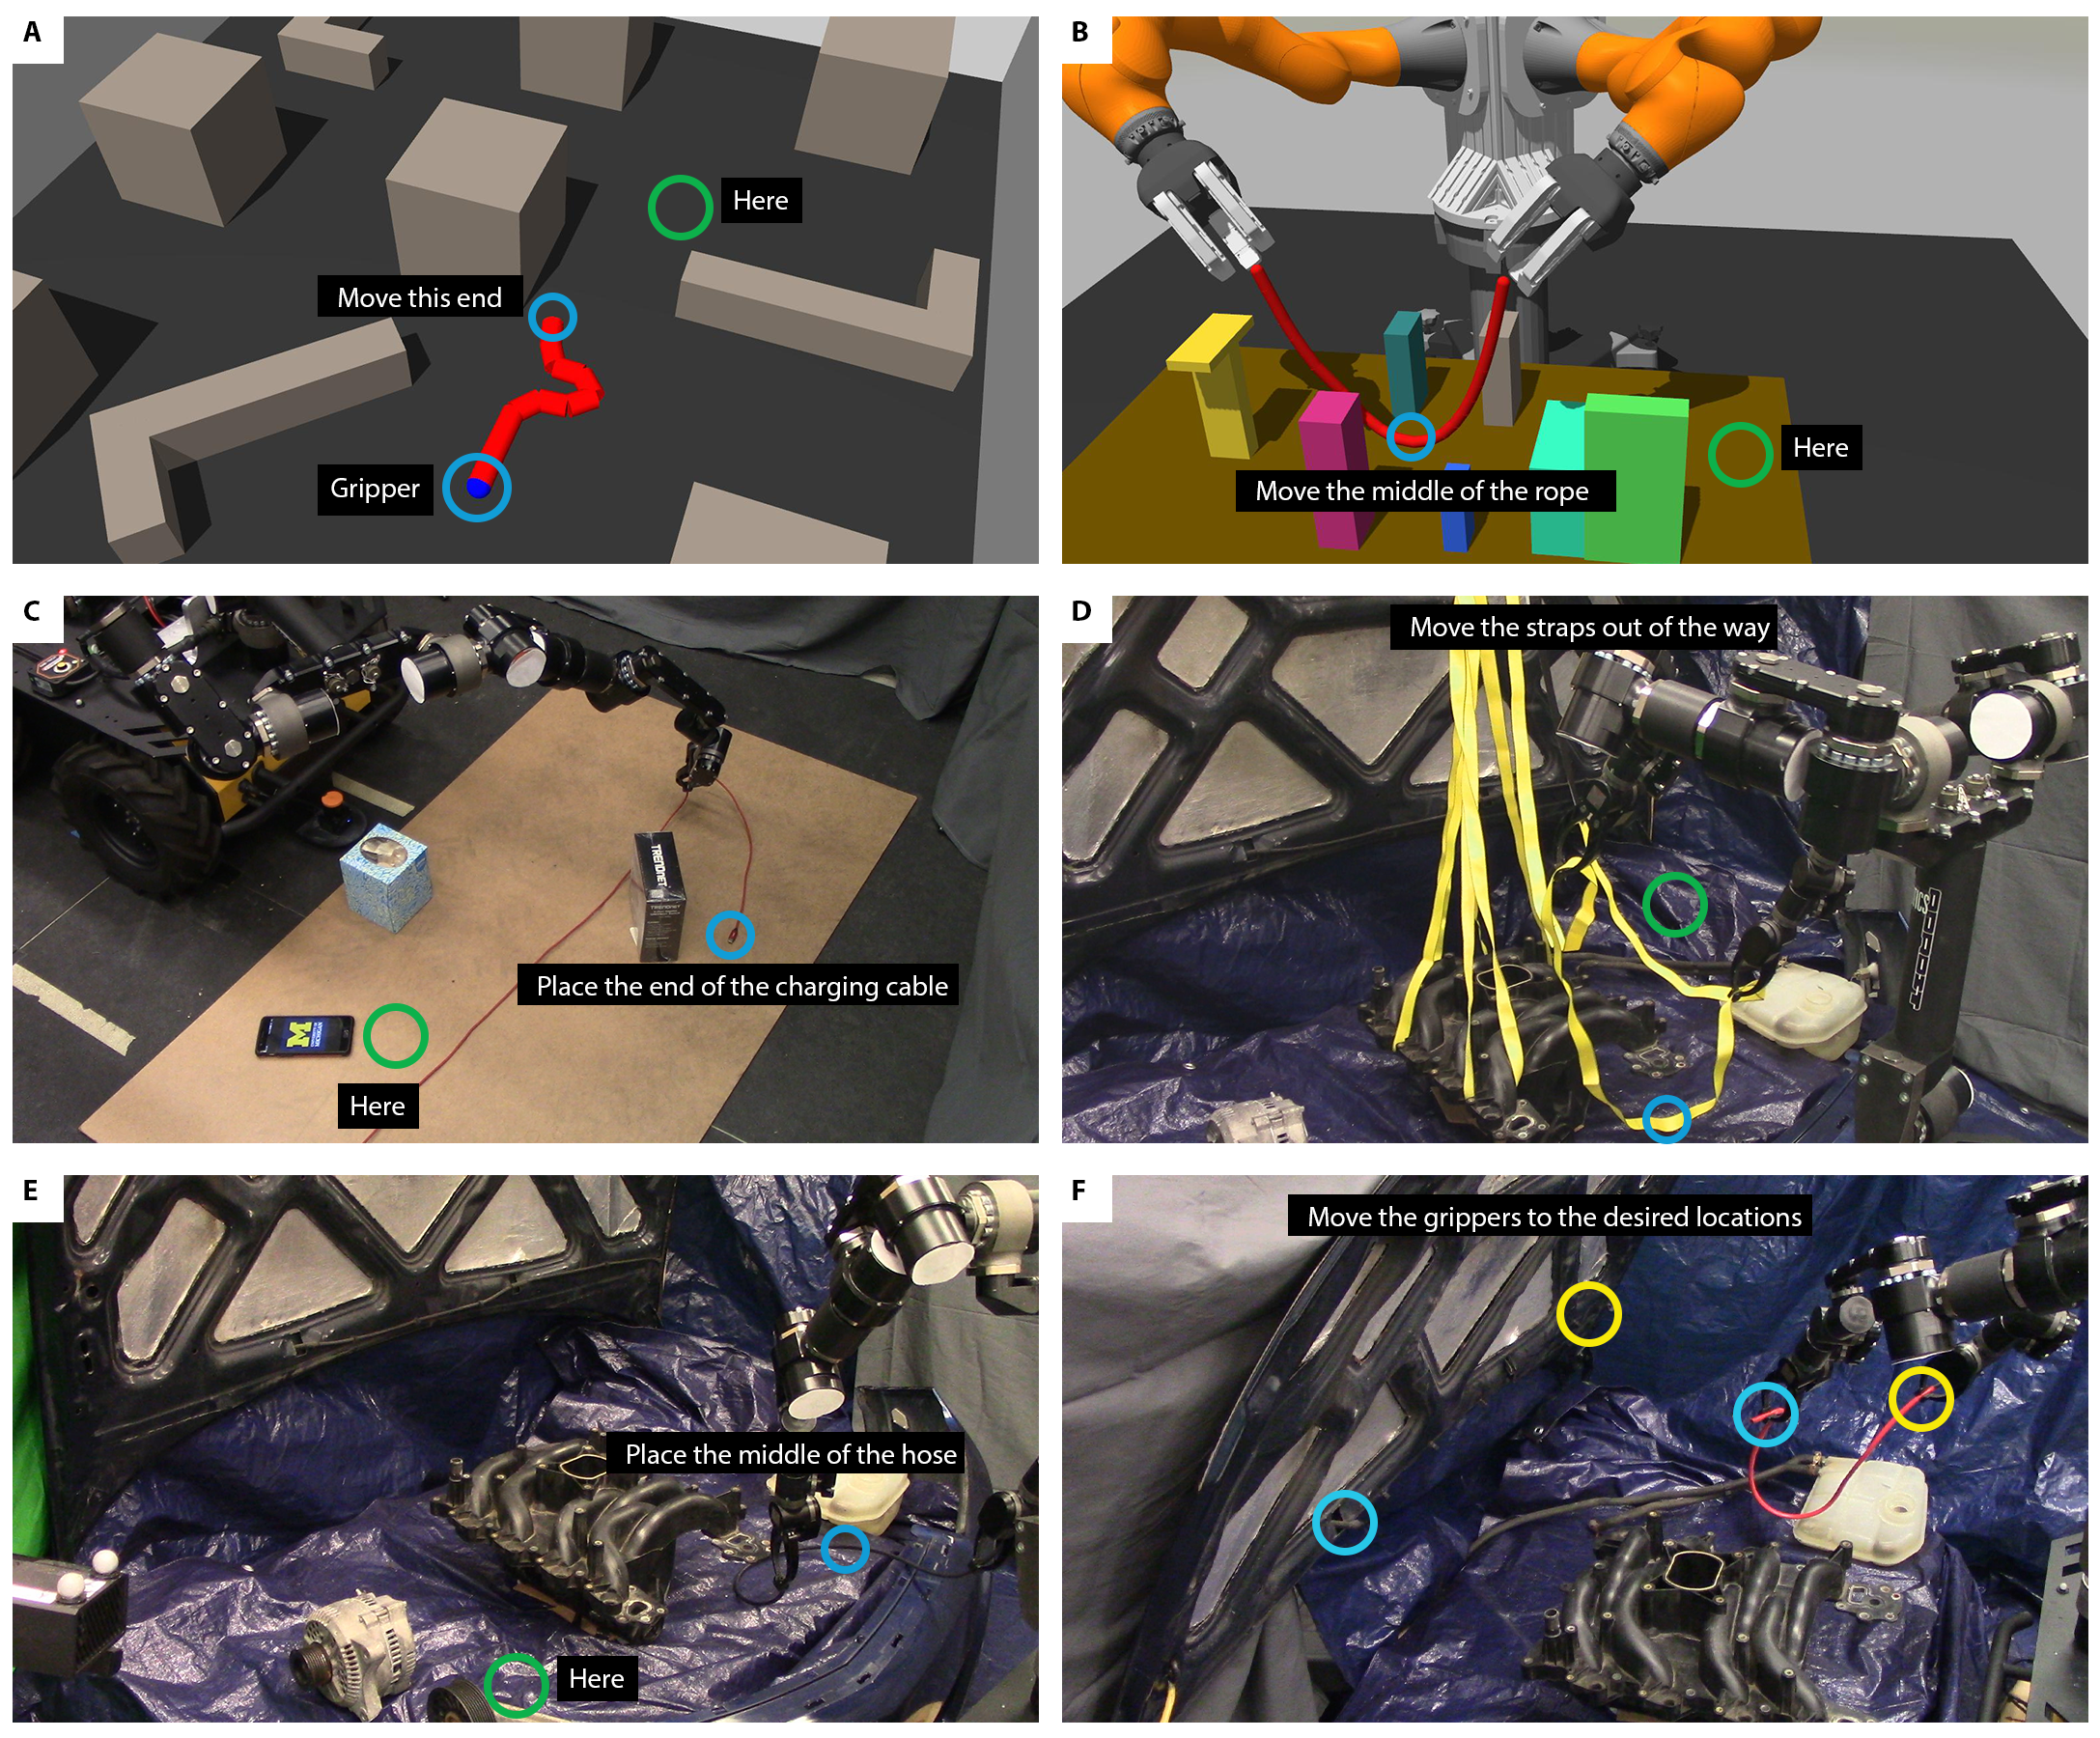
\includegraphics[width=0.8\linewidth]{Chap2/images/figure2}
    \caption{Pictures of our simulation and real robot scenarios. (A) Simulated Rope Dragging. (B) Simulated Tabletop Rope Manipulation. (C) Retrieving a Charging Cable. (D) Removing Lifting Straps. (E) Moving a Hose. (F) Preparing to Install a Hose. Annotations show examples of goals for various tasks our method can complete.}
    \label{Scirob:fig:figure2}
\end{figure}


\subsection{Data Collection for Learning the Dynamics}

\label{Scirob:sec:phase_one_collection}
Our first phase of data collection is used for training our model of the unconstrained dynamics. This involves sampling random actions and recording the observed states to form trajectories $[\state^0,\action^0,\state^1,\dots,\lasttrainaction,\lasttrainstate]$. In all our experiments, we use $\trainhorizon=10$. We sample actions randomly, choosing target positions which are within \SI{0.1}{\meter} of the current gripper position(s). Put another way, we sample actions which are changes in position in a ball around the current position. We repeat the previously sampled change in position with 80\% probability, which creates larger, more consistent motions and gives better coverage of our environments. During this phase, we do not reset the rope's position between trajectories.

In this phase, we also want to avoid activating physical constraints during data collection. This is done by removing obstacles, and by restricting the actions taken during data collection. For rope dragging, this only means removing any obstacles. For dual arm rope manipulation, this means removing obstacles, removing the arms entirely, and preventing the rope from overstretching by limiting the distance between the grippers. Although removing the arms would not be possible in the real world, it seems possible to design a conservative set of actions which would similarly ensure that the rope does not interact with the arms, or the arms with each other. At a high level, the purpose of this is to simplify the dynamics by avoiding activating any physical constraints during this phase.

For rope dragging, we collected 6,144 trajectories containing 10 steps, of which 1,536 are reserved for validation and testing. For dual arm rope manipulation, we collected 2,048 trajectories containing 10 steps, of which 512 are reserved for validation and testing.
\subsection{Learning the Unconstrained Dynamics}
\label{Scirob:sec:learning_dynamics}

Once we have collected our dataset of trajectories, we train our dynamics network. This network is a two layer fully connected neural network which takes in a state $\currentstate$ and action $\currentaction$ and predicts a change in state $\Delta \nextstatepred$. A diagram showing this architecture is shown in Figure \ref{Scirob:fig:figure4} and discussed in more detail in Section ``\nameref{Scirob:sec:architectures}''. This model can be used to make multistep predictions by feeding the predicted state back into the model. The loss is the combined prediction error for all time steps in the trajectory, and is shown in Equation \eqref{Scirob:eq:dyn_loss}.

\begin{equation}
	\begin{split}
	MSE(\state^0, \action^0, \dots, \lasttrainaction) &= \frac{1}{\trainhorizon} \sum_{t=1}^{\trainhorizon-1} \left\| \currentstatepred - \currentstate \right\|^2 \\
	\statepred^0 &= \state^0 \\
	\nextstatepred &= \ourdynamics(\env, \currentstatepred, \currentaction)
	\end{split}
	\label{Scirob:eq:dyn_loss}
\end{equation}

\subsubsection{Incorporating Uncertainty in the Learned Dynamics}
\label{Scirob:sec:uncertainty}

Prior work has shown that it can be beneficial to consider the uncertainty in the learned dynamics \cite{Schneider1996,Bechtle2019,Chua2018}, even without considering constraints not seen in training. For instance, if the training data does not cover the state-action space well, then having a measure of uncertainty in the dynamics predictions makes it possible to detect out of distribution predictions. This is a measure of \textit{epistemic uncertainty}---uncertainty due to lack of data (as opposed to inherent randomness) \cite{Hullermeier2021,Hora1996}.

As is done in prior work \cite{Gal2016,Chua2018,Lakshminarayanan2017}, we use an ensemble of neural networks trained on the same phase one data starting with different random seeds. When a point prediction is needed, like in planning or in constructing the classifier and recovery datasets, we take the mean of the ensemble prediction. When a measure of uncertainty is needed, we compute the sum of the standard deviations along each dimension of state across all the models in the ensemble. For simplicity we will denote this as $\variance$. We use this measure of uncertainty as an input to the classifier. The intuition behind this method is that the trained networks' predictions will be similar near the training data, but will diverge far away from training data. This makes it possible for the classifier to reject or accept transitions based on the uncertainty of the learned dynamics. Although we did not find that this provided a significant improvement for our tasks, we include it nonetheless as it may be beneficial in scenarios where the unconstrained model is trained on a dataset with poor coverage of the state space.

\subsection{Phase Two Data Collection}
\label{Scirob:sec:phase_two_collection}

Once the unconstrained dynamics have been learned, we next learn where this model is accurate, and what actions to take when it is not. For this, we perform a second phase of data collection. In this phase, we collect data in the kinds of environments where we intend to perform tasks. We perform the same type of random data collection process as in the first phase, but now physical constraints are included, allowing us to gather examples of where our unconstrained dynamics are accurate and where they are not. Using the data collected in this phase, we can construct datasets to train our classifier as well as our recovery actions model. A related approach was used in \cite{Guzzi2020} for learning to estimate the reachability of a quadruped robot. Our prior work has also demonstrated that this type of data can also be collected by planning and executing those plans, rather than by taking random actions \cite{McConachie2020}. However, both of the above methods used analytical/simulation models for predicting the dynamics. Furthermore, our approach is in contrast to many methods in robust control and safe reinforcement learning, which are built on the idea that predictions made outside the training distribution are unreliable \cite{Zhou1998,Gal2016}. Those methods do not require a second data collection phase, but as a consequence would be overly conservative as the presence of any obstacle near the rope would be considered out-of-distribution.

In order to get diverse data we frequently randomize the locations of obstacles in the environment. For dual arm rope manipulation, this requires releasing the rope and moving the arms out of the way before randomizing obstacles, so that we can arrange the obstacles without permanently entangling the rope or arms.

For rope dragging, we collected 2,048 trajectories of length 50 in phase two, of which 512 were reserved for validation and testing. For dual arm rope manipulation, we collected 5,996 trajectories of length 20, of which 1,516 were reserved for validation and testing.

In total, the combined phase one and two datasets for dragging has 163,840 transitions, and the combined phase one two datasets for dual arm rope manipulation has 140,400 transitions. In comparison, \cite{Propnet} uses 500,000 transitions in order to accurately learn the contact dynamics of a rope amongst disc-shaped obstacles in 2D.

\subsection{Learning the Classifier}
\label{Scirob:sec:learning_classifier}

Given the data collected in phase two, we now describe how to construct training examples for the classifier. For this we need both the predictions of the unconstrained dynamics as well the labels of whether the model-error requirement is satisfied. To compute the predictions, we take the starting state for each trajectory in the dataset and roll out the unconstrained dynamics prediction for the rest of the trajectory. This produces a tuple of $(\currentstate, \currentstatepred, \currentaction, \nextstate, \nextstatepred)$ for each time step in each trajectory. As stated in Problem $\eqref{Scirob:eq:planning_problem}$ the label should be 1 if $\modelerrorconstraint$ and 0 otherwise. To compute $\modelerror$, we require a distance function $\distfname$ between the predicted state $\nextstatepred$ and the actual state $\nextstate$. We selected the threshold $\modelerrorthreshold$ by computing the 90th percentile of prediction error for the unconstrained dynamics on the unconstrained dynamics validation set. A sensitivity analysis of the threshold is given in Supplementary Materials. For rope dragging, $\modelerrorthreshold=$\SI{0.065}{\meter} and for dual arm rope manipulation $\modelerrorthreshold=$\SI{0.025}{\meter}. Additionally, we discard all the transitions after the first transition labeled 0, since it is unclear whether the dynamics would have been accurate had it not diverged previously. A diagram illustrating how a trajectory is converted into examples for the classifier is shown in Figure \ref{Scirob:fig:3DClassifierInput}.

\begin{figure}
    \centering
    \includegraphics[width=0.6\linewidth]{Chap2/images/figure5}
    \caption{Representing the state and environment in 3D voxel grids. (A) An example for rope dragging. (B) An example dual arm rope manipulation. Different colors are used to represent different channels in the voxel grid, and alpha is used to indicate the voxel value, with 0 being fully transparent and 1 being fully opaque.}
    \label{Scirob:fig:3DClassifierInput}
\end{figure}

The classifier network $\classifierdef$ takes as input the environment $\env$ and the transition $\currentstatepred,\currentaction,\nextstatepred$. Since we use an ensemble of dynamics models, these states are the mean predictions of the ensemble. We also include the variance $\variance$ of the ensemble predictions as input to the classifier. The classifier outputs a number between 0 (inaccurate) and 1 (accurate). The network architecture is shown in Figure \ref{Scirob:fig:figure4}. Since this is a binary classification problem, we use binary cross-entropy loss to train it. Furthermore, since physical constraints are spatial in nature, we convert the environment and states into multi-channel 3D voxel grids and use Convolutional Neural Networks (CNN) (details in Section ``\nameref{Scirob:sec:architectures}'').

We also note that depending on the environments and specific parameters for how actions are sampled, the resulting dataset of transitions may be imbalanced. In our experiments, our classifier datasets contained more positive than negative examples, ranging between 65\% and 95\% positive. To mitigate bias in our classifier, we balance each minibatch by oversampling examples from the underrepresented class.

\subsection{Planning With a Learned Model and Classifier}
\label{Scirob:sec:planning}

Once we have learned our unconstrained dynamics and classifier, these models are used for planning. Although they could be applied to a number of different planning methods, including the cross entropy method (CEM) \cite{Kobilarov2011}, probabilistic roadmaps (PRM) \cite{Kavraki1996}, or trajectory optimization \cite{Ratliff2006}, we chose to use them in a kinodynamic RRT \cite{LaValle2001}, as implemented in the Open Motion Planning Library (OMPL) \cite{ompl}. Kinodynamic RRT is a sampling-based tree-search algorithm, and is well suited for our tasks as they contain local minima and narrow passages. Graph-based methods like PRMs could be used instead if we expect to plan repeatedly in the same environment, and trajectory optimization could be used if there are criteria such as path length which should be minimized.

In our Kinodynamic RRT, we sample a single random action $\currentaction$ and attempt to extend using that action. Whenever we attempt to extend from state $\currentstatepred$ with action $\currentaction$ to the state $\nextstatepred$, we first check the transition $(\currentstatepred,\currentaction,\nextstatepred)$ by feeding it through the classifier. The extension is added to the tree only if the classifier output is greater than $\paccept$. We chose this type of planner for its simplicity, and many algorithmic and implementation optimizations could be made to decrease planning times.

\subsection{Evaluating Stuck States and Learning Recovery}
\label{Scirob:sec:learning_recovery}

The formal definition of being stuck (Equation \eqref{Scirob:eq:recovery}) evaluates every possible action from a given state. In practice, checking whether a state is stuck consists of sampling $\NRecoverySamples$ actions and checking whether any of them are accepted by the classifier. Since the classifier is trained to approximate the MER, this is a quick and effective method for determining whether recovery is needed. Additionally, this procedure is done naturally by the RRT at the start of planning, which means that checking for recovery can be easily integrated into planning without any redundant calls to sampling, dynamics, or classification.

Given the unconstrained dynamics and the classifier, we can also use the data collected in phase two to learn recovery actions. As defined in our problem statement, recovery actions are needed when the robot is in a state where the classifier rejects all proposed actions. In this case, we would like the robot to take \textit{recovery actions} which bring it back to regions of state space where the unconstrained dynamics are accurate.

For this, we propose training a neural network to evaluate the probability that an action is recovering. This network takes in a state, action, and the environment $\recovInputs$ and outputs the probability $\recovProb$ that the action is recovering. Specifically, when we detect recovery is needed, we sample $\NRecoverySamples$ actions randomly and use this learned recovery model to assign each action a probability of recovering. The highest probability action is then selected and executed; this sampling, recovery probability evaluation, and execution process repeats until the system is no longer stuck. This approach requires training a model which estimates the probability that an action is recovering. To construct a dataset of recovering actions and labels of the recovery probability, we use a similar approach to the one used to construct the classifier dataset.

This process considers each observed transition $\currentstate,\currentaction,\nextstate$ and environment $\env$ in the dataset and first determines whether recovery is needed at $\currentstate$. We sample $\NRecoverySamples$ random actions from that state, predict according to the unconstrained dynamics, and feed this into the classifier. If all $\NRecoverySamples$ sampled transitions are rejected, then the state $\currentstate$ needs recovery. Next we perform the same test starting at the next state $\nextstate$. Here we record the proportion of the sampled actions which were accepted, and this is used as the label for probability of recovery $\recovProb$. For example, if at $\currentstate$ none of the random samples were accepted, but from $\nextstate$ all $\NRecoverySamples$ were accepted, then this is an excellent example of recovery, and we would like our recovery model to predict that taking action $\currentaction$ from $\currentstate$ in environment $\env$ is likely to lead to recovery. On the other hand, if when checking $\nextstate$ we find that still no actions are accepted by the classifier, then this is a poor example of recovery. We use all transitions for which recovery is needed (i.e. $\recoveryfuncfull = 1$ as the dataset for training our recovery model, and train the network using binary-cross entropy to predict the recovery probability. For our experiments, we set $\NRecoverySamples$ to 32. More details about the neural network and its structure can be found in Section ``\nameref{Scirob:sec:architectures}''.

Approaches to recovery like those from the safe exploration community \cite{Koller2018,Berkenkamp2017,Fisac2019safety} are focused on staying within a region of the state space from which the agent can guarantee safety during the learning process, or the existence of a sequence of control actions which will move the system into a predefined safe set. In contrast, our method is targeting the case where the model is already too unreliable for use at the given state and any predictions made cannot be trusted.

\subsection{Network architectures}
\label{Scirob:sec:architectures}

\begin{figure}
    \centering
    \includegraphics[width=0.7\linewidth]{Chap2/images/figure4}
    \caption{Network architectures. (A) dynamics, (B) classifier, and (C) recovery. \textit{local} refers to the translations used to make the states and actions invariant to the position in the world frame, and is described in Sections ``\nameref{Scirob:sec:learning_dynamics}'', ``\nameref{Scirob:sec:learning_classifier}'', and ``\nameref{Scirob:sec:architectures}''. Green capsules shapes indicate vectors, and blue boxes indicate functions. The gray 3D box represents the 3D voxel grid representation of state (Section ``\nameref{Scirob:sec:voxels}'').}
    \label{Scirob:fig:figure4}
\end{figure}

Our method uses three neural networks, one for the dynamics model, one for the classifier, and one for recovery. Architectures are shown in Figure \ref{Scirob:fig:figure4}.

\subsubsection{Dynamics Model Architecture}

The dynamics network is a two layer fully connected network with 1,024 hidden units in each layer and ReLU activation. This model takes in the state of the rope and grippers concatenated with the actions and outputs the change in state, which is then added to the input state to produce the final predicted state. Furthermore, because we assume that the unconstrained dynamics are invariant to the global position in space, we first translate the state and actions into a local frame before feeding them into the dynamics network. For rope dragging, states and actions are relative to the position of the gripper, and for dual arm manipulation they are relative to the average of all the points of the rope. 

\subsubsection{Classifier Architecture}

The classifier network takes in the environment $\env$ and a transition $\transitionpred$ and outputs the probability of the MER being satisfied. Since we experimented with performing classification on multiple transitions we use a Long Short Term Memory network (LSTM) with a CNN encoder, although in this work we only consider a single transition as input. As shown in Figure \ref{Scirob:fig:figure4}, a single time step is passed through a CNN encoder that maps a single state $\currentstatepred$ and action $\currentaction$ into a latent vector. The state and environment are first represented in a 3D voxel grid and passed through three convolutional layers. The output is flattened and concatenated with the vector representations of the state and action. The LSTM outputs a scalar prediction of the probability of the MER being satisfied for each time step. Since we use a single transition, this means there are two outputs, one for time $t$ and one for $t+1$. The output for time $t$ is ignored, because it is not a function of $\nextstatepred$. Instead, we use the output for time $t+1$ as the probability for the entire transition $\transitionpred$.

\label{Scirob:sec:voxels}
In order to represent the environment and states in a voxel grid of a fixed size, we take a crop of the full environment occupancy grid centered around the local origin (as defined above for dynamics). As with the local representation of states and actions, this assumes invariance to the absolute position. Additionally, using a fixed size local environment has the benefit of allowing the size of the full environment to change from task to task without any retraining. In order to make it easier for the classifier to reason over the 3D input, we also include a 3D representation of the input states. For each component of the state (grippers, rope) we construct a 3D voxel grid of the same size and location as the local environment and each voxel's value is proportional to the inverse-log of its distance to the nearest point in that component of the state. This results in a smoothed version of simply drawing the points into the voxel grid, and examples are shown in Figure \ref{Scirob:fig:3DClassifierInput}. We stack these representations along with the local environment to get a multi-channel voxel grid.

The vector representations of state and action are the same as is described for the dynamics, however we use both the original state vector (not translated) and the local state vector (translated). This is because the classifier should be able to learn reachability and kinematic constraints, e.g. in our dual-arm manipulation scenario. 

\subsubsection{Recovery Architecture}

Finally, the recovery network has the same encoder structure as the classifier, and we use the learned parameters, without fine-tuning, of convolution layers from the classifier in the recovery network. This network takes in a proposed transition, this time consisting of the 3D local environment, a single state, and a proposed action, and outputs the probability of recovery. Unlike the classifier, we do not pass in the predicted result of the proposed action, since recovery is only used when accurate predictions cannot be made. After encoding, two fully connected layer with ReLU activation followed by a layer with sigmoid activation are used to map down to the output probability.

\subsubsection{Full Dynamics Architecture}

Our full dynamics baseline uses a different network. We use the network proposed in \cite{NagabandiImageConditiondDynamics2018}, but extend to 3D convolution. The state representations used are the same as in our unconstrained dynamics network. Graph neural network architectures for predicting physics in 3D may provide more accurate predictions \cite{Propnet,Mrowca2018}, however these networks assume a graphical model of the world is known, whereas our dynamics learning method does not.

\subsection{Simulation Environments}
\label{Scirob:sec:sim_envs}

We use the Gazebo simulator with ODE physics \cite{Gazebo,ODE} for our quantitative experiments. We emphasize that our method does not have access to the simulator's model of the rope or the simulation parameters. For our rope dragging experiment, the rope is modeled with 10 rigid links, and the state consists of the positions of the links and the position of the gripper $\state=[x_g,y_g,z_g,x_1,y_1,z_1,\dots,x_{10},y_{10},z_{10}]$, which has 33 dimensions.
We considered including gripper orientation, however this would make the dynamics dependent on gripper geometry and friction properties (because the rope could wind around the gripper) without necessarily enabling significant new capabilities, so we chose not to include orientation. The gripper is attached to one end of the rope, and the point at the other end of the rope (which we will call the tail) is the point which we wish to place at a goal position. Task error is measured is the Euclidean distance in 3D between the tail and the goal point. The actions are target gripper positions $\action = [x,y,z]$, and a local controller is used to attempt to reach these goals. When commanded into an obstacle, the gripper will stop or potentially slide as it applies force into the obstacle. An action completes when the commanded position is reached or a timeout of 1 second occurs. The nominal joint velocity of the controller is tuned to reduce jerk and keep the simulation quasi-static.

For the dual arm rope manipulation experiments, the rope is modeled with 25 rigid links, and the state consists of the positions of the links and the positions of the two grippers $\state=[x_{g1},y_{g1},z_{g1},x_{g2},y_{g2},z_{g2},x_1,y_1,z_1,\dots,x_{25},y_{25},z_{25}]$, which has 81 dimensions.
The grippers attach to opposite ends of the rope. The actions are target positions for each gripper $\action = [x_1,y_1,z_1,x_2,y_2,z_2]$. A Jacobian-based inverse kinematics controller is used to track the target position for each gripper. This controller stops when the target position is reached or just before any collisions between the arms or between the arms and obstacles.
\section{Discussion} \label{SciRob:sec:discussion}

\subsection{On the Specialization to Deformable Objects}
Planning with inaccurate models has many potential applications, so it would be interesting to explore a broader range of tasks in future work. However, deformable object manipulation is particularly well-suited for our framework. Specifically because  1) Compliance allows us to make mistakes, stop, and replan; 2) Dynamics are more complex in some regions than in others; and 3) Much of the state space and dynamics are irrelevant for doing useful tasks. We discuss each of these points below:

First, our method relies on taking actions for which we have no accurate model, which means we must be able to take actions safely, despite their outcome being uncertain. The compliance afforded by deformable objects allows us to safely collect data, and thus to learn where our model is wrong.

Second, our method assumes that there is some subset of the dynamics which we can learn accurately, and which is sufficiently useful. Such an assumption is particularly well-suited to deformable object manipulation, where the full dynamics are much more difficult to learn than the unconstrained dynamics, yet interesting and practical tasks can still be done without learning these dynamics.

Third, deformable objects have high-dimensional state-action spaces. However, only a small region of state-action space is either reachable or useful for practical tasks (i.e. we need not consider the many different crumpled or knotted states). Because of this, it is often acceptable to avoid large portions of this space. Our method takes advantage of this in many ways, including 1) only learning the dynamics for the subset of state-action space covered in phase 1 data collection, and 2) only learning the classifier for the relatively small subset of state-action space covered in phase 2 data collection.

\subsection{Limitations} In this work we present significant progress on planning with unreliable models and addressing their inaccuracies, however many open questions remain. In this work we do not address challenges in state estimation and tracking, control and precise manipulation, or in describing and defining complex tasks.

There are also many avenues in which our proposed methods might be improved or extended. For instance, we define which simplified dynamics should be learned by defining the phase one setting and data collection procedures. This assumes that we know which dynamics will be tractable to learn, but still useful for planning in more constrained scenarios. In future work, it would be interesting to explore how to make this decision automatically, e.g. we can search over various simplifications of the dynamics based on the performance of learned models. Finally, we plan to extend these methods to incorporate real world data based on potentially unreliable perception and tracking.

Although we show that our method can be used for several interesting tasks, we are limiting the tasks our method can do by choosing to learn only the unconstrained dynamics. Our method assumes that the goal is reachable while remaining in the part of state-action space where the unconstrained dynamics are accurate. While this is a reasonable assumption, it would be interesting to incorporate our method into a framework which uses it to get as close as possible to a given goal and then switching to a feedback-based local method (e.g. \cite{LinearAlarcon2013,Jia2018,Wu2020}) to finalize the task (as is done in \cite{McConachie2020}).

In terms of recovery, we note that although our learned recovery actions dramatically improved our performance for the dual arm manipulation task, the learned recovery policy still fails in some cases. The learned recovery policy tends to raise the grippers, as this is an effective strategy in the training data. However, while this will work well when the rope is draped on the table or obstacles, it leads to being caught on a protrusion if the rope starts below it. A better policy would likely be learned by collecting phase two data in environments where getting caught and escaping is more likely. 

In this work, we treat the simulator as a black-box proxy for the real world. However, these simulations can differ from real world physics, and so at best they provide a starting point from which sim2real methods can be used to transfer either a learned dynamics model \cite{Fu2016,Clavera2018} or a learned policy \cite{Bousmalis2018,Peng2018} to the real world. For instance, it would be useful to adapt online to different stiffnesses of lengths of rope without re-collecting large datasets. Sim2real has been demonstrated for a number of other robots and tasks \cite{Lee2020,OpenAI2019}, and incorporating these techniques into our proposed methods is an interesting direction for future work.
\subsection{Learning Performance}
In addition to reporting the performance of our complete method on various tasks, here we also report the training and validation accuracies of our learned models. Further details on the training of these models can be found in Sections ``\nameref{Scirob:sec:learning_dynamics}'', ``\nameref{Scirob:sec:learning_classifier}'', and ``\nameref{Scirob:sec:learning_recovery}''.

For dynamics learning, we report learning error as the Euclidean distance between every predicted and true point on the rope, and average over all the points, time steps, and examples in the dataset. For rope dragging, our unconstrained dynamics model has an error of \SI{0.0081}{\meter} in training and \SI{0.0097}{\meter} in testing. These numbers are small in comparison to the length of the rope (\SI{0.5}{\meter}) and the size of the environment (2x2m). For a visual demonstration of this level of error,r please see our video. FD achieves an error of \SI{0.0090}{\meter} in training and \SI{0.0117}{\meter} in testing. For dual arm rope manipulation, our unconstrained dynamics model has an error of \SI{0.0025}{\meter} in training in \SI{0.0030}{\meter} in testing. Here the rope has a length of \SI{0.8}{\meter}, indicating that we are able to learn the unconstrained dynamics very accurately. The full dynamics baseline achieves an error of \SI{0.0194}{\meter} in training and \SI{0.0218}{\meter} in testing. Learning accurate dynamics over long horizons is critical for planning, and by learning only the unconstrained dynamics, our method is able to do so with higher accuracy than the full dynamics baseline.

We report learning metrics on the phase two dataset (see Section ``\nameref{Scirob:sec:learning_classifier}'' for details). For rope dragging, the classifier achieved an accuracy of $0.890$, precision of $0.959$ and recall of $0.822$ on the training set. On the testing set, it has an accuracy of $0.835$, precision of $0.888$, and recall of $0.789$. For dual arm rope manipulation, the classifier achieved an accuracy of $0.904$, precision of $0.914$ and recall of $0.927$ on the training set. On the testing set, it has an accuracy of $0.890$, precision of $0.895$, and recall of $0.927$. Throughout our experimentation we observed that, as prior work has noted \cite{McConachie2020}, the accuracy of this classifier is a poor indicator of its usefulness in planning.

For recovery, we use the binary cross entropy loss to measure learning performance. For rope dragging, the training loss (unitless) is $0.021$ and the testing loss is $0.023$. For rope dragging, the training loss is $0.139$ and the testing loss is $0.146$. 

\subsection{Physical Robot Demonstrations}
\label{Scirob:sec:physical_robot_details}
To demonstrate the practicality of our method, we designed real-world mockups of domestic and automotive tasks. For dual arm manipulation, we demonstrate three tasks done under the hood of a car, where the robot manipulates hoses and straps. For rope dragging we show an example where the robot retrieves a phone charging cable by sliding it. For clarity and simplicity, we demonstrate only the parts of these tasks where our method applies and forgo the use of sophisticated local controllers to, for example, plug the charging cable into the phone.

Perception of deformable objects remains a difficult open problem \cite{Yan2020}, much less in cluttered environments where the object is partially-occluded. Online perception of the object is not within the scope of this paper. To demonstrate our methods despite not having such perception algorithms, we manually constructed the scenes in a simulator and planned our actions there before executing them on the real robot. In future work we will incorporate online perception into our execution pipeline when the appropriate perception algorithms are available.

In both scenes, we re-use the unconstrained dynamics models learned in simulation directly. For rope dragging, we also re-use the classifier and recovery models as-is. For dual arm manipulation however, because a different robot is used, and the scene geometry differs significantly from our simulation, we use classifier and recovery models trained on scenes similar to the one we test on in the real world.  For more information, see the video in our supplemental materials. 

\subsection{Experiment Design}
To compare these methods quantitatively, we consider the task error over 150 trials per method in two types of rope manipulation tasks. The obstacle configurations are randomized before every trial, and each trial is allowed 180 seconds. During these 180 seconds, the method alternates between action selection and execution, where action selection is either planning or recovery. The trial is terminated if the goal is reached or the time limit is reached (see Figure \ref{Scirob:fig:figure1}, and Supplementary Materials for more details).

At the end of the trial, the final state is used to determine task error, and we report statistics of this error across the trials. A trial is a success if the final state error is below the goal threshold. Because tasks are generated randomly, some tasks will be impossible to achieve (e.g. the object cannot reach the goal because of a barrier), thus the absolute success rate is less informative than the difference in success rates between methods. When claims of statistical significance are made, a one-sided T-test is used and p-values are reported.

\section{Results}

To rigorously evaluate our approach, we perform statistical comparisons of our method vs. ablations and baselines in simulation over two types of rope manipulation tasks in 150 randomly-generated environments. We show that our approach greatly improves performance over learning the full dynamics as well as simply trusting the model learned in a simplified setting. We then demonstrate the practicality of our method for performing tasks on a real robot in domestic and automotive scenarios.

\subsection{Baselines}

In this work we argue that learning the dynamics for deformable objects in environments with constraints such as obstacles is difficult, and that we should instead learn only the unconstrained dynamics and a classifier to predict when those dynamics are valid. To support this claim we compare to a method which plans with a model of the full dynamics. We term this baseline Full Dynamics (FD), and we learn the dynamics using an approach similar to \cite{Nagabandi2018} (see Section ``\nameref{Scirob:sec:learning_dynamics}''). In FD, we learn the dynamics from a dataset collected in the same way as we collect data for our classifier (Section ``\nameref{Scirob:sec:phase_two_collection}''). Our method uses two phases of data collection, the data in each phase is used differently. Therefore, to make a fair comparison, the full dynamics baseline is trained on a dataset whose size is equal to our method's two datasets combined. Once trained, we plan with FD using the same Rapidly-exploring Random Tree (RRT) planner as in our method. However, unlike our method, FD requires no constraint checker (learned or otherwise), as anything we might consider a constraint is subsumed by the dynamics.

Additionally, we remove various components of our method to demonstrate the benefits they provide. We compare to a version called \textit{No Classifier}, which plans using our unconstrained dynamics but no constraint checker. Comparisons to this baseline show the benefit of using the classifier over simply trusting the unconstrained dynamics everywhere. We also compare to a version without recovery (\textit{Classifier}), and a method which takes random actions as its recovery policy (\textit{Classifier + Random Recovery}).

\subsection{Scenario 1: Rope Dragging}
 
Here we describe our results for the task of dragging a rope-like object along a surface among obstacles, as is shown in Figure \ref{Scirob:fig:figure1}a. Rope manipulation has numerous important applications including suturing and managing wires or hoses, and the rope dragging task requires long horizon planning for which our method is well-suited. The task is to place one end of a rope at a point while dragging the rope by the other end. This task is difficult because the system is highly under-actuated and the environment is cluttered. Task error is the Euclidean distance between the end of the rope and the goal point. The goal region is a sphere about the goal point with radius \SI{5}{\centi\meter}. This task illustrates the challenges of long horizon planning for deformable objects in cluttered scenes, and is challenging for existing methods. The practicality of our method is illustrated in our physical robot demonstrations.

The task error across 50 trials is shown in Figure \ref{Scirob:fig:figure6}a. Our complete method reached the goal 76\% of the time with a mean task error of \SI{4.48}{\centi\meter}. This is better than FD (32\% success, \SI{20.32}{\centi\meter} error) and No Classifier (60\% success, \SI{8.20}{\centi\meter} error) and is significant at p $< 0.001$. Additional numerical results are shown in Table \ref{Scirob:tab:dragging_results}. For this task, recovery was never needed, meaning that for all states from which the planner was run there was at least one action from that state which our classifier accepted as yielding an accurate prediction. The benefit of recovery actions is shown in the dual arm manipulation task below.

To show the ability of our classifier to learn difficult prediction functions, we also compare our results to a manually-engineered solution for this scenario. By inspecting the data of where the model tended to make errors, we found that, unsurprisingly, the model could not predict the effect of pushing/pulling the rope into obstacles but was fairly accurate when not in contact with obstacles or sliding along them (See Supplementary Materials for examples of sliding motion accepted by our classifier). To capture this predictive behavior with a rough approximation we used a collision checker to measure if the predicted state was penetrating into the obstacle in place of our learned classifier (as is done in \cite{Lamiraux2001}). Note that this is a scenario-specific method derived by using human intuition and an engineered collision-checker. While this intuition and hand engineered solution can be an effective solution for some tasks, changes in the task or object being manipulated often lead to additional tuning and engineering. For example, if the rope was very thick and the points defining the rope state (which are along the central axis of the rope) did not enter obstacles even when the rope was pressing into an obstacle, collision boundaries would need to be tuned. Likewise, if the rope is very thin, numerical error in predictions could lead to erroneous collision-checking results when sliding along the surface of an obstacle. To the credit of our method, we found that using the collision checker gave a 78\% success rate and a mean task error of \SI{12.74}{\centi\meter}, with p $= 0.498$ for the hypothesis that our method outperforms the collision checking method. This is an encouraging result, as it demonstrates that our method can perform on-par with a scenario-specific human-engineered solution, at least in this scenario.

\subsection{Scenario 2: Dual Arm Rope Manipulation}

\begin{figure}
    \centering
    \begin{subfigure}[b]{0.49\textwidth}
        \centering
        \includegraphics[width=\textwidth]{Chap2/images/dragging_success.jpeg}
        \label{Scirob:fig:dragging_success}
    \end{subfigure}
    \hfill
    \begin{subfigure}[b]{0.49\textwidth}
        \centering
        \includegraphics[width=\textwidth]{Chap2/images/dual_success.jpeg}
        \label{Scirob:fig:dual_success}
    \end{subfigure}
    \caption{Comparing success across methods. (left) The success rate as a function of the success threshold on task error for our simulated rope dragging experiments. The dashed line indicates the size of the goal region used. For example, this tells us that if our goal region was \SI{0.1}{\meter}, the "Classifier" method would achieve about 84\% success. (right) The success rate as a function of the success threshold on task error for our simulated dual arm rope manipulation experiments.}
    \label{Scirob:fig:figure6}
\end{figure}

Here we describe our results for using a robot for dual arm manipulation of rope among obstacles, as is shown in Figure \ref{Scirob:fig:figure2}b. Using two arms to manipulate deformable objects allows more control of the object than one arm and introduces additional interesting challenges in coordinating the two arms. The task we use for evaluation is to place the midpoint of the rope at a point in 3D while only holding the ends. In addition to obstacles, this scenario imposes the constraints of not overstretching the rope, not colliding the arms, and staying within the reachability limits of the robot. Task error is the Euclidean distance between the midpoint of the rope and the goal point. The goal region is defined as a sphere about the goal point with radius \SI{5}{\centi\meter}. This type of manipulation, while difficult for existing methods, is a prerequisite for many practical tasks such as cable harnessing.

The task error across 100 trials is shown in Figure \ref{Scirob:fig:figure6}b. Our complete method (\textit{Classifier + Learned Recovery}) reached the goal 84\% of the time with a mean task error of \SI{7.29}{\centi\meter}. This is statistically significantly (p $<0.001$) better than FD, which reached the goal 17.7\% of the time with a mean task error of \SI{20.32}{\centi\meter}, and No Classifier, which reached the goal 47\% of the time with a mean task error of \SI{16.97}{\centi\meter}. We also compare to our method without recovery actions, and to our method with random recovery actions. In this task, recovery actions are critical, and without them our method performs statistically significantly (p $<0.001$) worse with a success rate of 61\% and a mean task error of \SI{14.69}{\centi\meter}. When compared to random recovery actions, which reaches the goal 78\% of the time, our method has similar task error (p $= 0.281$ for the hypothesis that our method outperforms random recovery), however our method needs only a third as many recovery actions to achieve this task error. Over all 100 trials, random recovery used 613 recovery actions whereas our method used only 177. Additional numerical results are shown in Table \ref{Scirob:tab:dual_results}.

\subsection{Physical Robot Demonstrations}
We demonstrate potential applications of our method on real-world mock-ups of several domestic and automotive tasks. The first set of tasks are performed under the hood of a car, and require the robot to manipulate straps or hoses. These tasks include moving the midpoint of a hose to a specific location (Figure \ref{Scirob:fig:figure2}e), positioning the ends of a wiper fluid hose for installation (Figure \ref{Scirob:fig:figure2}f), and removing lifting straps from an engine (Figure \ref{Scirob:fig:figure2}d).

We also perform the task of fetching a charging cable (Figure \ref{Scirob:fig:figure2}c). In this example, the robot cannot reach the end of the cable directly because it is blocked by an obstacle. Instead, the robot grasps the cable elsewhere, and must drag the end of the cable towards the phone.

Notably, these tasks use several different types of goals described in the state space of the rope and grippers, all of which can be handled by our planner. This is in contrast to policy learning methods \cite{matas2018sim2real,Sundaresan2020,Wu2020} and methods which use goal images \cite{Nair2017,Finn2017,Zhang2019}. More details on how we perform these tasks can be found in Section ``\nameref{Scirob:sec:physical_robot_details}''.

\FloatBarrier

\begin{table}
    \centering
    \begin{tabular}{lllccccc}
    \hline\noalign{\smallskip}
     Name                        & Dynamics      & Classifier  & \makecell{max\\(m)} & \makecell{mean\\(m)} & \makecell{median\\(m)} & \makecell{std. dev.\\(m)} \\
    \noalign{\smallskip}\hline\hline\noalign{\smallskip}
     \makecell[l]{Classifier}    & Unconstrained & Learned     & 1.133   & 0.128    &  0.044     & 0.247 \\
     \noalign{\smallskip}\hline\noalign{\smallskip}
     \makecell[l]{No Classifier} & Unconstrained & None        & 1.408   & 0.325    &  0.045     & 0.425 \\
     \noalign{\smallskip}\hline\noalign{\smallskip}
     \makecell[l]{Full Dynamics} & Full          & None        & 1.519   & 0.438    &  0.156     & 0.450 \\
    \noalign{\smallskip}\hline
    \end{tabular}
    \caption{\label{Scirob:tab:dragging_results} Task error statistics for simulated rope dragging.}
\end{table}

\begin{table}
    \centering
    \begin{tabular}{lllccccc}
    \hline\noalign{\smallskip}
     Name                                        & Dynamics      & Classifier  & \makecell{max\\(m)} & \makecell{mean\\(m)} & \makecell{median\\(m)} & \makecell{std. dev.\\(m)} \\
    \noalign{\smallskip}\hline\hline\noalign{\smallskip}
     \makecell[l]{Classifier\\Learned\\Recovery} & Unconstrained & Learned    & 0.450   & 0.073    &  0.045     & 0.094 \\
     \noalign{\smallskip}\hline\noalign{\smallskip}
     \makecell[l]{Classifier\\Random\\Recovery}  & Unconstrained & Learned    & 0.629   & 0.081    &  0.046     & 0.106 \\
     \noalign{\smallskip}\hline\noalign{\smallskip}
     \makecell[l]{Classifier}                    & Unconstrained & Learned    & 0.630   & 0.147    &  0.047     & 0.167 \\
     \noalign{\smallskip}\hline\noalign{\smallskip}
     \makecell[l]{No Classifier}                 & Unconstrained & None       & 0.741   & 0.170    &  0.082     & 0.165 \\
     \noalign{\smallskip}\hline\noalign{\smallskip}
     \makecell[l]{Full Dynamics}                 & Full          & None       & 0.621   & 0.203    &  0.191     & 0.142 \\
    \noalign{\smallskip}\hline\noalign{\smallskip}
    \end{tabular}
    \caption{\label{Scirob:tab:dual_results}Task error statistics for simulated dual arm rope manipulation.}
\end{table}
\section{Conclusion}

In summary, the proposed method is able to complete a variety of difficult rope manipulation tasks in clutter. We are able to learn the unconstrained dynamics accurately, and by using our learned classifier, the planner successfully avoids the regions of state-action space where these unconstrained dynamics are incorrect. Using the classifier outperforms both using the full dynamics and simply trusting the unconstrained model by a wide margin. Last, recovery makes the method more resilient, allowing the robot to act even when it cannot trust its dynamics model. In our tabletop manipulation simulations, we demonstrated that these recovery actions statistically significantly improve the success rate of our method.
 
\chapter{Data Augmentation for Learning Reliability}
\label{chap:DataAugmentation}
The previous chapter introduced the Model-Error Requirement RRT and a method for learning a recovery policy. In simulation, we used these methods to learn the reliability of a dynamics model for bimanual rope manipulation. We also executed trajectories planned in simulation in the real world to illustrate what it would look like to apply these methods in the real world. This was needed because the proposed learning methods did not consider data efficiency, and required datasets that would be impractical to collect in the real world.

This chapter address this problem, by proposing a data augmentation method for manipulation. We first formalize data augmentation as an optimization problem, where we attempt to maximize diversity, validity, and relevance. We propose loss functions that formalize these abstract concepts, and apply our proposed method to learning dynamics and learning reliability. Finally, we use the proposed data augmentation method to learn reliability for dual-arm rope manipulation -- online, from scratch, and in the real world.

\section{Introduction} \label{RSS:sec:introduction}

In recent years, interest in applying deep learning to robotic manipulation has increased. However, the lack of cheap data has proven to be a significant limitation \cite{DisbandOpenAI2021}. To enable applications such as smart and flexible manufacturing, logistics, and care-giving robots \cite{WEFRobots}, we must develop methods that learn from smaller datasets, especially if the learning is done online on real robots.

One of the simplest and most effective ways to mitigate the problem of small datasets is to use data augmentation. While data augmentation has been shown to significantly improve generalization performance in tasks like image classification, it is not straightforward to extend existing data augmentation methods to the types of data used in robotic manipulation. Furthermore, most existing augmentation methods fall into one of two categories, and both have severe limitations:

In the first category, augmentations are defined by a set of transformations, sampled independently for each example. Most image augmentation methods fall into this category, where rotations or crops are sampled randomly for each example \cite{Augerino2020,AutoAugment,BestPractice2003}. By making augmentations independent of the example being augmented, we are restricted to operations which are valid on all examples. In the second category, there are methods which learn a generative model (VAE, GAN, etc.) of the data, and then sample new training examples from that model \cite{BayesianDATran2017,MaterialsAEOhno2020,PriceForecastingAE2021}. This approach assumes a useful generative model can be learned from the given dataset, but we found these methods did not perform well when the dataset is small.

\begin{figure}
    \centering
    \includegraphics[width=0.9\linewidth]{Chap3/images/title_figure.png}
    \caption{A mock-up of a car engine bay. The robot must move the rope and place it under the engine without snagging it to set up for lifting the engine. We use data augmentation to improve task success rate during online learning for this task.}
    \label{RSS:fig:real_robot_setup}
\end{figure}

\begin{figure*}
    \centering
    \includegraphics[width=1\linewidth]{Chap3/images/rope_aug_examples.png}
    \caption{Examples of augmentations of rope generated by our method. On the left is a picture of the scene in simulation from a zoomed out viewpoint. The simplified engine block model is in the center. The rope start (dark blue) and end (light blue) states are shown, with the grippers shown at the start state. The static environment geometry is shown in brown. The first row shows a transition in free space, where the resulting augmentations are particularly diverse. The final augmentation shows how our method found a transformation to move the rope underneath the hook while remaining in free space. The second row shows a transition which involves contact between the rope and the environment. The augmentations preserve this contact.}
    \label{RSS:fig:rope_aug_examples}
\end{figure*}


It is not trivial to define a coherent framework for data augmentation that encompasses many domains and many types of learning problems (e.g. classification and regression). Thus, the first contribution of this chapter is a formalization of the data augmentation problem. In our problem statement (Section \ref{RSS:sec:problem}), we formalize data augmentation as an optimization problem based on three key criteria: \textit{validity}, \textit{relevance}, and \textit{diversity}. We define an augmented example as \textit{valid} if it obeys the laws of physics and is possible in the real world. Augmentations are \textit{relevant} if they are similar to data that would be seen when performing the target task. \textit{Diversity} encourages the augmentations to be as varied as possible, i.e. the transformations applied to the data should be uniformly distributed to maximize diversity. Producing diverse augmentations for each original example is key to improving the generalization of the trained network.

The general definitions of validity, relevance, and diversity we propose depend on information that is intractable to compute for many manipulation problems, and therefore we also present approximations to these definitions. We do not claim that this formulation is useful for all manipulation problems, and clearly define the physical assumptions behind this formulation in Section \ref{RSS:sec:problem}.

Our second contribution is a method for solving this approximated optimization problem. Our method operates on trajectories of object poses and velocities, and searches for rigid-body transformations to apply to the moving objects in the scene to produce augmentations. Our method encourages validity by preserving contacts and the influence of gravity. Additionally, we encourage relevance by initializing the augmentations nearby the original examples and preserving near-contacts. Finally, we encourage diversity by pushing the augmentations towards randomly sampled targets.

Our results demonstrate that training on our augmentations improves downstream task performance for a simulated cluttered planar-pushing task and a simulated bimanual rope manipulation task. The learning problems in these tasks include classification and regression, and have high-dimensional inputs and outputs. Lastly, we demonstrate our augmentation in an online learning scenario on real-robot bimanual rope manipulation using noisy real-world perception data (Figure \ref{RSS:fig:real_robot_setup}). In this scenario, augmentation increased the success rate from 27\% to 50\% in only 30 trials. Additional materials such as code and video can be found on our \href{https://sites.google.com/view/data-augmentation4manipulation}{project website}.

\section{Problem Statement}  \label{RSS:sec:problem}

In this section, we formally define the form of data augmentation studied in this chapter. We define a dataset $\dataset$ as a list of examples $\example\in\exampleSpace$ and, optionally, labels $\ell(\example)=\classLabel$, where $\ell$ is a task-specific labeling function. We assume the space $\exampleSpace$ is a metric space with a distance function $\distfname$. Augmentation is a stochastic function $\augDef$ which takes in an example $\example$ and produces the augmented example $\exampleAug$. The general form is shown in Algorithm \ref{RSS:alg:aug_prototype}. Internally, augmentation will call \sample{} to generate a vector of parameters, which we call $\transform$. We also define $\exampleAugSet$ as a set of $k$ augmented examples produced by calling \sample{} then \apply{} $k$ times. The parameters $\transform$ describe the transformation which will be applied to the example in the \apply{} procedure. We focus on augmentation functions that are stochastic, thus $\augf$ will sample new augmented examples each time it is called. If the dataset contains labels $\classLabel$, we assume that the labels should not change when the example is augmented.

\begin{algorithm}[t]
\caption{$\augf(x)$}\label{RSS:alg:aug_prototype}
$\transform = \sample{}(\example) $\\
$\aug{\example} = \apply(\example,\transform)$\\
return $\aug{\example}$\\
\end{algorithm}

We propose that useful augmentations should be \textit{valid}, \textit{relevant}, and \textit{diverse}. Let the valid set $\validSet$ be the set of examples which are physically possible. Let the relevant set $\relevantSet$ be the set of examples likely to occur when collecting data for or executing a specific set of tasks in a specific domain. We define $\mathrm{validity}(\exampleAug)=1$ if $\exampleAug \in \validSet$ and $\mathrm{validity}(\exampleAug)=0$ otherwise. We also define $\mathrm{relevance}(\exampleAug):=e^{-\distf{\exampleAug}{\relevantSet}}$ and $\mathrm{diversity}(\exampleAugSet):=\uniformity$, where $\klF$ is the Kullback–Leibler divergence and $\transformDist$ is the distribution of the parameters for a set of augmented examples $\exampleAugSet$. Diversity is maximized when the augmentation transformations are uniformly distributed in the range $\transformUniformRange$. With these concepts defined, we define data augmentation as the following optimization problem, the solution to which is a set of augmentations $\exampleAugSet$:

\begin{equation}
    \label{RSS:eq:most_general}
    \begin{array}{cc}
        \underset{\exampleAugSet}{\mathrm{max}} & \mathrm{diversity}(\exampleAugSet) + \beta \sum_{\exampleAug_i}\mathrm{relevance}(\exampleAug_i) \\
        \mathrm{subject\: to} & \mathrm{validity}(\exampleAug_i)\:\:\quad \forall\,\exampleAug_i \in \exampleAugSet\\
        & \ell(\aug{\example})=\ell(\example) \\
    \end{array}
\end{equation}

\noindent where $\beta$ is a positive scalar.

This optimization problem can be solved directly if $\validSet$, $\relevantSet$, and $\ell$ are known. However, in manipulation tasks, that is rarely the case. Instead, we will formulate an approximation to this problem using measures of relevance, diversity, and validity that are derived from physics and useful for a variety of robotic manipulation tasks and domains.

\begin{figure}
    \centering
    \includegraphics[height=5cm]{Chap3/images/car_sim_env-cropped.png}
    \includegraphics[height=5cm]{Chap3/images/cylinders_env.png}
    \caption{(left) The environment for bimanual rope manipulation, in simulation. (right) The environment for cluttered planar pushing of cylinders, in simulation.}
    \label{RSS:fig:sim_envs}
\end{figure}

\subsection{Assumptions}
\label{RSS:sec:assumptions}

Most augmentation algorithms rely on some expert knowledge or heuristics to define what is a valid augmentation. For instance, rotating an image for image classification makes an assumption that rotation does not change the label, and this is not always true. Similarly, the efficacy or correctness of our algorithm is also subject to certain assumptions. Here, we define the key assumptions:

\begin{itemize}
    \item The geometry of the robot and all objects is known.
    \item The scene can be decomposed into objects which can be assigned or detected as either moving or stationary.
    \item Examples are time-series, consisting of at least two states.
    \item All possible contacts between stationary vs. moving objects have the same friction coefficient.
    \item Contacts between the robot and objects/environment (e.g. grasps) can be determined from the data.
    \item A rigid-body transformation of an object preserves internal forces arising from its material properties.
    \item Objects only move due to contact or under the force of gravity. We do not handle movement due to magnetism or wind, for example.
\end{itemize}

Notably, the assumption that a rigid-body transformation preserves internal, material forces is what allows us to handle cluttered scenes with many moving objects, as well as deformable or articulated objects. While it could be valuable to augment the deformation or relative motion of the objects, doing so in a way that is valid would be challenging. Instead, we transform them all rigidly (See examples in Figures \ref{RSS:fig:rope_aug_examples},\ref{RSS:fig:cylinders_aug_examples}).

The assumption of having a common friction coefficient between all moving versus stationary objects is in-line with much manipulation research. For example, work on planar pushing assumes friction is uniform across the plane \cite{PushSim2021,PushYu2016}. Note that we make no assumption on the coefficients of friction between two moving objects.

Naturally, there are scenarios where these assumptions do not hold and thus where our algorithm may not perform well. However, our experiments demonstrate significant improvement on two very different manipulation scenarios, and we expect these assumptions extend to other scenarios as well.
\section{Methods} \label{RSS:sec:methods}

We first describe an approximation to the augmentation problem \eqref{RSS:eq:most_general}, which is specialized for manipulation. Next, we decompose this problem and describe each component in detail.

\subsection{Algorithm Overview}

Since robotic manipulation is interested specifically in moving objects, we focus on augmenting trajectories of poses and velocities of moving objects. A key insight is that objects in the scene can be categorized as either robots, moved objects, or stationary objects, and that these should be considered differently in augmentation. We denote the moved objects state as $\state$, the robot state as $\robot$, the robot action as $\action$, and the stationary objects as $\env$ (also called environment). Our method augments the moved object states, the robot state, and the actions, but not the stationary objects. We do not assume any specific representation for states or actions, and examples of possible representations include sets of points, joint angles, poses, or joint velocities. Since we operate on trajectories, we bold the state ($\bm{\state},\bm{\robot}$) and action ($\bm{\action}$) variables to indicate time-series (e.g $\state_{1:T}=\bm{\state}$). With this categorization, we can write $\example=\{\bm{\state},\bm{\robot},\bm{\action},\env\}$ and $\aug{\example}=\{\bm{\aug{\state}},\bm{\aug{\robot}},\bm{\aug{\action}},\env\}$.


We choose the parameters $\transform$ to be rigid body transformations, i.e. either $SE(2)$ or $SE(3)$. We parameterize $\transform$ as a vector with translation and rotation components, with the rotation component with Euler angles bounded from $-\pi/2$ to $\pi/2$, which gives uniqueness and a valid distance metric. These rigid body transforms are applied to moved objects in the scene, and augmented robot state and action are computed to match. We choose rigid body transforms because we can reasonably assume that even for articulated or deformable objects, augmenting with rigid body transforms preserve the internal forces, and therefore the augmentations are likely to be valid.

It may seem that an effective method to generate augmentations is then to randomly sample transforms independent of the data. However, this is not an effective strategy because it is highly unlikely to randomly sample valid and relevant transformations. We confirm this in our ablations studies (included in the Appendix 1.A). Instead of sampling transforms randomly, we formulate an approximation to Problem \ref{RSS:eq:most_general}:

\begin{equation}
    \label{RSS:eq:method}
    \begin{array}{cc}
        \underset{\transform}{\mathrm{min}} & 
        \lossDiversity(\transform,\target{\transform}) +
        \betaBbox\lossBbox(\bm{\aug{\state}}) + \betaValid\lossValid(\transform) + \\
        & \betaOcc\lossOcc(\bm{\aug{\state}},e) + \betaDmd\lossDmd(\bm{\aug{\state}},\env) + \\
        & \lossRobot(\bm{\aug{\state}},\bm{\aug{\robot}},\bm{\aug{\action}},\env) \\[1em]
        \text{subject to} & \{\bm{\aug{\state}},\bm{\aug{\robot}},\bm{\aug{\action}},\env\} = \apply(\bm{\state},\bm{\robot},\bm{\action},\env,\transform) \\
        & \target{\transform}\sim\transformUniform \\
    \end{array}
\end{equation}

The decision variable is now the parameters $\transform$, and the validity constraint is moved into the objective. We propose that diversity should be maximized by the transforms being uniformly distributed, and therefore $\lossDiversity$ penalizes the distance to a target transform $\target{\transform}$ sampled uniformly within $[\transform^-,\transform^+]$. The relevance and validity terms (which are intractable to compute) are replaced with four objective functions, which are specialized to manipulation. The magnitudes of different terms are balanced by ${\betaBbox,\betaValid,\betaOcc,\betaDmd}$, which are defined manually. We define each objective function below:

\subsubsection{Bounding Box Objective}
First is the bounding-box objective $\lossBbox$, which keeps the augmented states $\bm{\aug{\state}}$ within the workspace/scene bounds defined by $[\state^-,\state^+]$. The bounding box objective encourages relevance, since states outside the workspace are unlikely to be relevant for the task.

\begin{equation}
\lossBbox = \sum_{i=1}^{|s|}{\max(0,\bm{\aug{\state}}_i - \state^+_i) + \max(0,\state^-_i-\bm{\aug{\state}}_i)}
\end{equation}

\subsubsection{Transformation Validity Objective}
The transformation validity objective $\lossValid$ assigns high cost to transformations that are always invalid or irrelevant for the particular task or domain. It is defined by function $\validF$, which takes in only the transformation. For example, in our rope manipulation case, it is nearly always invalid to rotate the rope so that it floats sideways. In our cluttered pushing task, in contrast, this term has no effect. This term can be chosen manually on a per-task basis, but we also describe how a transformation validity objective can be learned from data in section \ref{RSS:sec:learnValid}.

\begin{equation}
\lossValid = \validF(\transform)
\end{equation}

\subsubsection{Occupancy Objective}
The occupancy objective $\lossOcc$ is designed to ensure validity by preventing objects that were separate in the original example from penetrating each other and ensuring that any existing penetrations are preserved. In other words, we ensure that the occupancy $O(p)$ of each point $\augStatePoint\in\augStatePoints$ in the augmented object state matches the occupancy of the corresponding original point $\statePoint\in\statePoints$. For this term, we directly define the gradient, which moves $\augStatePoint$ in the correct direction when the occupancies do not match. This involves converting the environment $\env$ into a signed-distance field (SDF) and the moved objects states $\bm{\state}$ into points $\statePoints$. This objective assumes that the environment has uniform friction, so that a contact/penetration in one region of the environment can be moved to another region.

\begin{equation}
\lossOcc=\sum_{\substack{\statePoint\in\statePoints \\ \augStatePoint\in\augStatePoints}} \SDF(\augStatePoint)\big(O(\statePoint)-O(\augStatePoint)\big)
\end{equation}

\subsubsection{Delta Minimum Distance Objective}
The delta minimum distance objective is designed to increase relevance by preserving near-contact events in the data. We preserve near-contact events because they may signify important parts of the task, such as being near a goal object or avoiding an obstacle. We define the point among the moved object points $\statePoints$ which has the minimum distance to the environment $\pointMinDist=\mathrm{argmin}_{\statePoint}\SDF(\statePoint)$. The corresponding point in the augmented example we call $\augPointMinDist$.

\begin{equation}
\lossDmd = ||\SDF(\pointMinDist)-\SDF(\augPointMinDist)||^2_2
\end{equation}


\begin{figure}
    \centering
    \includegraphics[width=0.5\linewidth]{Chap3/images/step_project.png}
    \caption{Illustration of \augState{} within Algorithm \ref{RSS:alg:aug}. All points and sets are in the space of $\transform$. The path of $\transform$ is shown in red with black arrows. The pink set, State Valid, is the set where \textit{state\_valid} is true. $\transform$ begins at the origin, and alternates between moving towards $\target{\transform}$ and projecting back into the set \textit{state\_valid} (by solving Equation \eqref{RSS:eq:project}).}
    \label{RSS:fig:step_project}
\end{figure}

\subsubsection{Robot Contact Objective}

The robot contact objective $\lossRobot$ ensures validity of the robot's state and the action. This means that contacts involving the moved objects which existed in the original example must also exist in the augmented example. Let the contact points on the robot be $\contactpoint_{\robot}$ and the contact points on the moved objects' state be $\contactpoint_{\state}$.

\begin{equation}
\lossRobot=\sum_i(||{\contactpoint_{\robot,i} - \contactpoint_{\state,i}}||^2_2)
\end{equation}

Finally, we note that other objective functions can be added for the purpose of preserving task-specific labels, i.e. so that $\ell(\example)=\ell(\aug{\example})$. However, for our experiments, no additional functions were necessary.

\subsection{Solving the Augmentation Optimization Problem}

This section describes how we solve Problem \eqref{RSS:eq:method}, and the procedure is detailed in Algorithm \ref{RSS:alg:aug}. First, we split the problem into two parts, \augState{} and \augRobot{}.

\begin{algorithm}[t]
\caption{$\augf(\bm{\state},\bm{\robot},\bm{\action},\env)$}\label{RSS:alg:aug}
\SetKwComment{Comment}{// }{}
\Comment{\augState{}}
$ \target{\transform} \sim \transformUniform $\\
$\transform = \mathbf{0}$ \text{ (identity)} \\
\For{$i \in \nStep$}{
    $\transform_\text{old}=\transform$ \\
    $\transform = \texttt{step\_towards}(\transform, \target{\transform})$ \\
    $\transform = $ solve Equation \eqref{RSS:eq:project} \\
    \If{$\distf{\transform} {\transform_\text{old}}<\projectionNotProgressing$}{
        break\\
    }
}
\Comment{\augRobot{}}
$\bm{\aug{\state}}, \textit{state\_valid} = \applyState(\bm{\state},\bm{\action},\transform)$\\
$\bm{\aug{\robot}},\bm{\aug{\action}}$, \textit{ik\_valid} $\leftarrow \mathrm{IK}(\bm{\robot},\bm{a},\bm{\aug{\state}},\env)$\\
\uIf{$!$state\_valid or $!$ik\_valid}{
    return $\bm{\state},\bm{\robot,}\bm{\action},\env$\\
}
\Else {
    return $\bm{\aug{\state}},\bm{\aug{\robot}},\bm{\aug{\action}},\env$\\
}
\end{algorithm}

In \augState{}, we optimize the transform $\transform$ to produce the moved objects' state $\bm{\aug{\state}}$ while considering environment $\env$. To achieve diversity, we uniformly sample a target transform $\target{\transform}$ and step towards it iteratively. This stepping alternates with optimizing for validity and relevance. We visualize this procedure in Figure \ref{RSS:fig:step_project}, as well as in the supplementary video. The innermost optimization problem is 
\begin{equation}
    \label{RSS:eq:project}
    \begin{array}{cc}
        \underset{\transform}{\mathrm{argmax}} & \betaBbox\lossBbox+\betaValid\lossValid+\betaOcc\lossOcc+\betaDmd\lossDmd \\
    \end{array}
\end{equation}

We solve Problem \eqref{RSS:eq:project} using gradient descent, terminating after either $\mProj$ steps or until the gradient is smaller than some threshold $\projStepSizeThreshold$.

Note that we start \augState{} in Algorithm \ref{RSS:alg:aug} with $\transform$ at the identity transformation, rather than initially sampling uniformly. This has two benefits. First, the identity transform gives the original example, which is always in the relevant set. Second, it is unlikely that a uniformly sampled transformation is valid or relevant, so starting at a random transformation would make solving Problem \eqref{RSS:eq:project} more difficult.

In \augRobot{}, we are optimizing $\lossRobot$. This corresponds to computing the augmented robot states $\bm{\aug{\robot}}$ and actions $\bm{\aug{\action}}$ given the augmented states $\bm{\aug{\state}}$ and the environment $\env$. Minimizing $\lossRobot$ means preserving the contacts the robot makes with the scene, which we do with inverse kinematics (Line 10 in Algorithm \ref{RSS:alg:aug}).

\subsection{Learning the Valid Transforms Objective}
\label{RSS:sec:learnValid}

As discussed above, we include a term $\lossValid$ based only on the transformation $\transform$. In some cases, such as our rope manipulation example, it may not be obvious how to define this objective manually. Our rope is very flexible, and therefore rotating the rope so that it floats in a sideways arc is invalid, but it may be valid for a stiff rope or cable. To address this, we offer a simple and data efficient algorithm for learning the transformation validity function $\validF$.

Our method for learning $\validF$ is given in Algorithm \ref{RSS:alg:valid_transformations_data}. This algorithm repeatedly samples augmentations of increasing magnitude, and tests them on the system (lines 6 and 8). This generates ground truth states starting from an input state and action. The result is a dataset $\learnValidDataset$ of examples ($\transform$, $\learnValidError$). We then train a small neural network $\learnedValidF$ to predict the error $\learnValidError$ and use the trained model as our transformation validity objective. We collect $\nLearnValid = \sqrt{10^\transformDim}$ examples, where $\transformDim$ is the dimensionality of the space of the transformation $\transform$.

\begin{algorithm}[t]
\caption{Data Collection for Learning Valid Transformations}\label{RSS:alg:valid_transformations_data}
\SetKwComment{Comment}{/* }{ */}
\KwIn{$\learnValidStateActionSet,\nLearnValid$}
\KwOut{$\learnValidDataset$}
$\minLearnValidError = \infty$ \\
\For{$i \in [1, \nLearnValid]$}{
    \For{$(\state_t,\robot_t,\action_t,\env) \in \learnValidStateActionSet$}{
        $ \learnValidScaling = i / \nLearnValid $ \\
        $ \transform \sim \mathbb{U}[\learnValidScaling\transform^-,\learnValidScaling\transform^+] $\\
        $ \state_{t+1}, \robot_{t+1} = \learnValidSimF(\state_t, \robot_t, \action_t, \env)$ \\
        $ \aug{\state}_{t,t+1}, \aug{\robot}_{t,t+1}, \aug{\action}_{t} = \apply(\state_{t,t+1},\robot_{t,t+1},\action_{t},\transform)$ \\
        $ \test{\aug{\state}_{t+1}}, \test{\aug{\robot}_{t+1}} = \learnValidSimF(\aug{\state_t}, \aug{\robot_t}, \aug{\action}_t, \env)$ \\
        $\learnValidError = || \aug{\state}_{t+1} - \test{\aug{\state}_{t+1}} ||$ \\
        \If {$\learnValidError < \minLearnValidError$}{
            $\minLearnValidError = \learnValidError,\,\transform_\text{min} = T,\,\minLearnValidError = \learnValidError$ \\
        }
    }
    add $(\transform_\text{min}, \minLearnValidError)$ to $\learnValidDataset$ \\
}
return $\learnValidDataset$
\end{algorithm}

This method owes its efficiency and simplicity to a few key assumptions about the system/data. First, we assume that we can collect a few ($<1000$) examples from the system and test various transformations. This could be performed in a simulator, as we do in our experiments. Because the transformation validity objective is not a function of state, action, or environment, we can make simplifications to this simulation by picking states and environments which are easy to simulate. We denote this set of states and actions as $\learnValidStateActionSet$. Second, because the transformation parameters are low-dimensional (3 and 6 in our experiments) the trained model generalizes well with relatively few examples.

\subsection{Application to Cluttered Planar Pushing}

In this section, we describe how we apply the proposed method to learning the dynamics of pushing of 9 cylinders on a table (Figure \ref{RSS:fig:sim_envs}). The moved object state $\state$ consists of the 2D positions and velocities of the cylinders. The robot state $\robot$ is a list of joint positions, and the actions $\action$ are desired end effector positions in 2D. There is no $\classLabel$ in this problem. The parameters $\transform$ used are $SE(2)$ transforms. In this problem, any individual trajectory may include some moved cylinders and some stationary ones. In our formulation, the stationary cylinders are part of $\env$ and are not augmented, whereas the moved ones are part of $\state$ and are augmented. The robot's end effector (also a cylinder) is also augmented, and IK can be used to solve for joint configurations which match the augmented cylinders' state and preserve the contacts between the robot and the moved cylinders.

\subsection{Application to Bimanual Rope Manipulation}

In this section, we describe how we apply the proposed method to a bimanual rope manipulation problem (Figure \ref{RSS:fig:sim_envs}). In this problem, there is a binary class label, so $\classLabel\in\{0,1\}$, which is preserved under our augmentation (last constraint in Problem \eqref{RSS:eq:most_general}). The rope is the moved object, and its state $\state$ is a set of 25 points in 3D. The robot state $\robot$ is a list of the 18 joint positions, and the actions $\action$ are desired end effector positions in the robot frame. In this problem, we know that the only contacts the robot makes with the objects or environment are its grasps on the rope. Therefore, we preserve these contacts by solving for a robot state and action that match the augmented points on the rope. The parameters $\transform$ used are $SE(3)$ transforms.

\begin{figure*}
    \centering
    \includegraphics[width=1\linewidth]{Chap3/images/cylinders_aug_examples.png}
    \caption{Examples of augmentations generated for learning the dynamics of planar pushing of 9 cylinders. The pink cylinder is the robot. Time is indicated by transparency. Augmentation transforms the positions and velocities of the cylinders that moved, including the robot. All moved objects are transformed together, rigidly. Despite the clutter, we are able to find relatively large transformations that still preserve existing contacts but do not create any new ones.}
    \label{RSS:fig:cylinders_aug_examples}
\end{figure*}
\section{Results} \label{RSS:sec:results}

We start by describing the tasks and our experimental methodology, then we present our results. These experiments are designed to show that training on augmentations generated by our method improves performance on a downstream task. We perform two simulated experiments, where we run thousands of evaluations, including several ablations (see Appendix 1.A). We also perform a real robot experiment (Figure \ref{RSS:fig:real_robot_setup}) where we run 30 iterations of online validity classifier learning, with augmentation and without. In all experiments, we train until convergence or for a fixed number of training steps. This ensures a fair comparison to training without augmentation, despite the differing number of unique training examples. In all experiments, we generate 25 augmentations per original example (See Appendix 1.B). We define key hyperparameters of our method in Appendix 1.C. A link to our code is available on the \href{https://sites.google.com/view/data-augmentation4manipulation}{project website}.

\subsection{Cluttered Planar Pushing}

\begin{figure}
    \centering
    \includegraphics[width=0.7\linewidth]{Chap3/images/cylinders_results1.png}
    \caption{Mean position error (meters) for learning the dynamics of cluttered planar pushing.}
    \label{RSS:fig:cylinders_results}
\end{figure}

The cluttered planar pushing environment consists of a single robotic arm pushing 9 cylinders around on a table. The task is to learn the dynamics, so that the motion of the cylinders can be predicted given initial conditions and a sequence of robot actions. For this, we use PropNet \cite{Propnet}, and our task is inspired by the application of PropNet to planar pushing in \cite{DBRP2020}. The inputs to PropNet are an initial state $\state_0$ and a sequence of actions $\baction$, and the targets are the future state $(\state_1,\dots,\state_T$). All trajectories are of length 50. We evaluate the learned dynamics by computing the mean and maximum errors for position and velocity on a held-out test set. Example augmentations for this scenario are shown in Figure \ref{RSS:fig:cylinders_aug_examples}. 

This is an interesting application of our augmentation for several reasons. First, it is a regression task, which few augmentation methods allow. Second, the output of the dynamics network is high-dimensional (900 for a prediction of length 50), which normally means large datasets are needed and engineering invariances into the data or network is difficult. Finally, the trajectories contain non-negligible velocities and are not quasi-static.

\begin{figure}
    \centering
    \includegraphics[width=0.6\linewidth]{Chap3/images/cylinders_rollouts.png}
    \caption{Predictions (blue) vs. ground truth (red) for planar pushing. The robot is in pink. Trajectories are visualized with lines. The left column shows predictions from a model trained with augmentation, the right column without.}
    \label{RSS:fig:cylinders_rollouts}
\end{figure}

The original dataset contained 60 trajectories of length 50, or \SI{3000} time steps in total. For comparison, previous work on the same dynamics learning problem used over \SI{100000} time steps in their datasets \cite{Propnet,DBRP2020}. This is similar to the number of training examples we have \textit{after} augmentation, which is \SI{75000} time steps. Finally, we measured the performance of our implementation and found that for the planar pushing scenario we generate 4.5 augmentations per second on average.

The primary results are shown in Figure \ref{RSS:fig:cylinders_results}. Augmentation reduces the average position error from \SI{0.00154}{\meter} to \SI{0.00133}{\meter}, a decrease of 14\%. Additionally, we include two baselines, one which adds Gaussian noise to the state, robot, action, and environment data, and one which uses a VAE to generate augmentations as in \cite{MaterialsAEOhno2020}. The magnitude of the Gaussian noise was chosen manually to be small but visually noticeable. Our proposed augmentation method is statistically significantly better than the baseline without augmentation ($p<0.0362$), the Gaussian noise baseline ($p<0.0001$), and the VAE baseline ($p<0.0002$). This difference in error may seem small, but note that error is averaged over objects, and most objects are stationary. Two roll-outs from with-augmentation and from without-augmentation are shown in Figure \ref{RSS:fig:cylinders_rollouts}. In particular, we found that augmentation reduces ``drift,'' where the model predicts small movements for objects that should be stationary. Finally, we note that the Gaussian noise and VAE baselines perform worse than no augmentation, suggesting that data augmentation can hurt performance if the augmentations are done poorly.

\subsection{Bimanual Rope Manipulation}

In this task, the end points of a rope are held by the robot in its grippers in a scene resembling the engine bay of a car, similar to \cite{UnreliableMitrano2021}, and shown in Figure \ref{RSS:fig:sim_envs}. The robot has two 7-dof arms attached to a 3-dof torso with parallel-jaw grippers. The tasks the robot performs in this scene mimic putting on or taking off lifting straps from the car engine, installing fluid hoses, or cable harnesses. These tasks require moving the strap/hose/cable through narrow passages and around protrusions to various specified goal positions without getting caught. One iteration consists of planning to the goal, executing open-loop, then repeating planning and execution until a timeout or the goal is reached. The goal is defined as a spherical region with \SI{4.5}{\centi\meter} radius, and is satisfied when any of the points on the rope are inside this region.

The planner is an RRT with a learned constraint checker for edge validity (validity classifier), and more details are given in \cite{UnreliableMitrano2021}. We want to learn a classifier that takes in a single transition $x = (\state_t,\action_t,\state_{t+1},\env_t)$ and predicts whether the transition is valid. Without a good constraint checker, the robot will plan trajectories that result in the rope being caught on obstacles or not reaching the goal. We apply our augmentation algorithm to the data for training this constraint checker. After an execution has completed, the newly-collected data along with all previously collected data are used to train the classifier until convergence. Example augmentations for this scenario are shown in Figure \ref{RSS:fig:rope_aug_examples}. The objective is to learn the constraint checker in as few iterations as possible, achieving a higher success rate with fewer data.

\begin{figure}
    \centering
    \includegraphics[width=1\linewidth]{Chap3/images/success_rate_rolling.png}
    \caption{The success rate on simulated bimanual rope manipulation, using a moving window average of 10.}
    \label{RSS:fig:rope_results}
\end{figure}

In this experiment, a total of \SI{3038} examples were gathered (before augmentation, averaged over the 10 repetitions). Since the purpose of our augmentations is to improve performance using small datasets, it is important that this number is small. In contrast, prior work learning a similar classifier used over \SI{100000} examples in their datasets \cite{UnreliableMitrano2021,UnreliableDale2019}. This is similar to the number of training examples we have \textit{after} augmentation, which is \SI{75950} on average.  Finally, we measured the performance of our implementation and found that for the rope scenario we generate 27 augmentations per second on average.

The primary results are shown in Figure \ref{RSS:fig:rope_results}. Over the course of 100 iterations, the success of our method using augmentation is higher than the baseline of not using augmentation, as well as the Gaussian noise baseline. We omit the VAE baseline, since it performed poorly in the planer pushing experiment. Furthermore, it is computationally prohibitive to retrain the VAE at each iteration, and fine-tuning the VAE online tends to get stuck in bad local minima. The shaded regions show the 95th percentile over 10 runs. If we analyze the success rates averaged over the final 10 iterations, we find that without augmentation the success rate is 48\%, but with augmentation the success rate is 70\%. The Gaussian noise baseline has a final success rate of 31\%. A one-sided T-test confirms statistical significance ($p<0.001$ for both).

\subsection{Real Robot Results}
\label{RSS:sec:real_robot_results}

\begin{figure}
    \centering
    \includegraphics[width=0.7\linewidth]{Chap3/images/real_robot_task_error_success.png}
    \caption{The success rate and task error distribution of bimanual rope manipulation on the real robot. Task error is the distance between the goal and the final observed state of the rope.}
    \label{RSS:fig:real_robot_results}
\end{figure}

In this section, we perform a similar experiment to the simulated bimanual rope manipulation experiment, but on real robot hardware. This demonstrates that our method is also effective on noisy sensor data. More importantly, it demonstrates how augmentation enables a robot to quickly learn a task in the real world. We use CDCPD2 \cite{CDCPD2} to track the rope state. The geometry of the car scene is approximated with primitive geometric shapes, like in the simulated car environment.

We ran the validity classifier learning procedure with a single start configuration and a single goal region, both with and without augmentation. After 30 iterations of learning, we stop and evaluate the learned classifiers several times. With augmentation, the robot successfully placed the rope under the engine 13/26 times. Without augmentation, it succeeded 7/26 times. The Gaussian noise and VAE baselines performs poorly in simulated experiments, therefore we omit them in the real robot experiments.

\section{Limitations} \label{RSS:sec:limitations}

First, our proposed method uses many hyper-parameters which may be difficult to tune. However, there are methods which can be used to automatically tune these parameters \cite{Augerino2020,AutoAugment}.

Additionally, there are problems and applications where the proposed objective functions do not ensure validity, relevance, and diversity. In these cases, the structure of our augmentation and projection procedures can remain, while new objective functions are developed. Another limitation is that our method is not compatible with image data. Much recent research in robotics has moved away from engineered state representations like poses with geometric information, and so there are many learning methods which operate directly on images. Although this is a limitation of the proposed method, many of the augmentations developed for images are also not applicable to problems in manipulation, even when images are used. For instance, pose detection, 3D reconstruction, semantic segmentation, and many other tasks may not be invariant to operations like cropping, flipping, or rotating. Creating an augmentation method for manipulation that is applicable to images is an open area for future research.

\section{Conclusion}  \label{RSS:sec:conclusion}

This paper proposes a novel data augmentation method designed for trajectories of geometric state and action robot data. We introduce the idea that augmentations should be valid, relevant, and diverse, and use these to formalize data augmentation as an optimization problem. By leveraging optimization, our augmentations are not limited to simple operations like rotation and jitter. Instead, our method can find complex and precise transformations to the data that are valid, relevant, and diverse. Our results show that this method enables significantly better downstream task performance when training on small datasets. In simulated planar pushing, augmentation decreases the prediction error by 14\%. In simulated bimanual rope manipulation, the success rate with augmentation is 70\% compared to 47\% without augmentation. We also perform the bimanual rope manipulation task in the real world, which demonstrates the effectiveness of our algorithm despite noisy sensor data. In the real world experiment, the success rate improves from 27\% to 50\% with the addition of augmentation.


 
\chapter{Focused Adaptation of Unreliable Dynamics}
\label{chap:FOCUS}
The previous chapter introduced a data augmentation method for manipulation. We used this method to learn reliability for dual-arm rope manipulation in from real world data. The dynamics model used in these experiments was also trained on real world data, in a separate phase that was designed to ensure no contact between the rope and the environment. This extra step was time-consuming and hand-designed, and attempts to use free-space dynamics pretrained in simulation failed because the simulation and the real world rope dynamics were too different.

This chapter address this problem, by proposing a novel dynamics adaptation method. Our key insight is that a free-space data from simulation is far more similar to free-space data from the real world than it is to non-free-space data from the real world. More generally, the problem we address is to adapt a dynamics model from a source environment to a target environment, where the source and target dynamics are similar in some regions but different in others. Our proposed adaptation method focuses adaptation on data where the dynamics are similar, which we show leads to more accurate dynamics for planning and good estimates of the dynamics model's reliability. Ultimately, we use this method to simultaneously adapt a dynamics model learned in simulation and learn reliability -- all online and in the real world.

\section{Introduction} \label{ICRA:sec:intro}

 Learning dynamics models for manipulation is an increasingly popular paradigm, in part because learned models can be repeatedly improved using autonomously collected real-world data. However, fine-tuning an initial dynamics model on new data can perform poorly when the data contains complex dynamics on which the dynamics model was not initially trained. For example, suppose we want to manipulate a rope amongst clutter, and we have a dynamics model trained on free-space motions in simulation. Free-space transitions in the real world are fairly similar to the free-space in simulation, but transitions where the rope deforms on objects in the scene are very different from anything seen in simulation. We call these transitions \emph{distracting}, because they are hard to learn from a few examples, and because they make it harder to adapt accurately to the free space dynamics. More generally, transitions from regions of dissimilar dynamics can inhibit effective transfer to regions of similar dynamics. This problem is similar to ``cleaning'' data in machine learning \cite{mislabeled99,filtering21,anomoly22}. For dynamics learning, defining what ``clean'' means can be difficult, and has not been studied extensively. Instead, the dominant paradigm is simply to train on all the collected data.

However, training on all the data can fail because real world datasets for learning dynamics are often too small to learn generalized models over the entire state-action space. In our experiments, we show that simply fine-tuning on all the data can yield a model that is not accurate enough for planning. If the task can be completed while remaining in regions where dynamics are similar, then it can be worth trading accuracy in dissimilar regions for accuracy in similar regions.
Our key insight is that, when we are adapting from an initial model, we can leverage the initial model to achieve significantly lower prediction error by focusing on transitions where the source and target dynamics are the most similar. The idea that transfer is easier when the source and target data are similar is well-supported in the transfer learning literature ~\cite{sorocky2020experience,bocsi2013alignment}. Concurrent work in offline reinforcement learning has also explored how staying closed to similar data leads to better policies \cite{vuong2022dasco}.

\begin{figure}
    \centering
    \includegraphics[width=1\linewidth]{Chap4/images/title_figure.pdf}
    \caption{
    (A) An illustration of how our adaptation method focuses on regions where the source and target dynamics are similar. When focusing adaption on free-space dynamics, the prediction errors decrease for other free-space data (similar), do not decrease for collision dynamics (dissimilar).
    (B) A mock-up of a car engine bay. The robot must move the rope and place it under the engine without snagging it to set up for lifting the engine. We use our proposed adaptation method to improve success rate during online learning for this task.}
    \label{ICRA:fig:real_robot_setup}
\end{figure}

To implement this strategy, we propose an adaptation method which minimizes prediction error in regions where the source and target dynamics are similar. The proposed method minimizes prediction error in these regions by fine-tuning on an initially small set of data from these regions, and growing that subset over the course of training. This is done with a loss function inspired by curriculum-learning that weighs transitions according to their prediction error, assigning higher weight to low-error transitions. Under the assumption that there are paths to the goal where the source and target dynamics are similar, this adaptation method can be used to achieve high task success in the target environment.

The first contribution of this chapter is a method for adapting dynamics models to datasets which contain distracting transitions. We demonstrate the proposed method is successful in filtering out distracting data and that the resulting trained model is more accurate in the regions of state-action space where the source and target dynamics are similar. The second contribution is a data-efficient online-learning method that pairs our adaptation method with prior work on planning with unreliable dynamics models \cite{UnreliableMitrano2021,MDEs22}. We call our combined method for online learning \FOCUS{}. \FOCUS{} achieves higher success rates in the low-data regime because the adapted dynamics are more accurate, which leads to finding more reliable plans.
\section{Problem Statement} \label{ICRA:sec:problem_statement}

The problem addressed in this chapter is to adapt a dynamics model trained in a source environment to data collected in a target environment, where the source and target environments have dynamics which are similar in some regions of the state-action space, but different in others. Furthermore, we consider the case where data collection is done by planning and executing paths to goals in the target environment using the learned dynamics model.

To formalize this, first consider the standard dynamics learning problem with a dataset $\dataset$ of transitions of states, actions, and next states $\transition$. We also assume a distance function $\distf{\state_1}{\state_2}$ that returns a scalar is given. The true dynamics are $\state'=\dynamics(\state,\action)$, and the learned dynamics are $\pred{\state}'=\learnedDynamics(\state,\action)$. We propose defining the source and target environment dynamics as similar for a transition if $\distf{\sourceDynamics(\state,\action)}{\targetDynamics(\state,\action)} < \softFilteringThrehsold$. The threshold $\softFilteringThrehsold$ should be small enough that it excludes distracting transitions, but large enough to include as much data from the target environment as possible. Let $\DST$ be the set of transitions from the target environment where this similarity condition holds.

In order to minimize the amount of data needed for adaptation to generalize, we aim to adapt the dynamics only to transitions from regions where this similarity condition holds ($\DST$). However, we also care about successfully completing the task, and therefore we also assume there are paths $\traj$ to the goal $\state^T\in\goal$ within the regions of similar dynamics $(\state^t,\action^t,\state^{t+1}) \in \DST $.

While the ultimate objective of adaptation should be to maximize task success in the target environment, an important condition for task success is minimizing prediction error on $\DST$. If the goal is reachable within $\DST$ (as we assume), the prediction error on $\DST$ is small (our objective), and our motion planner is constrained to stay in $\DST$, then we can also expect high task success. Next, we discuss how our adaptation method minimizes error on $\DST$, followed by how we can achieve high task success by additionally constraining a motion planner to $\DST$.

\begin{figure}
    \centering
    \includegraphics[width=1\linewidth]{Chap4/images/overview_diagram.pdf}
    \caption{Block diagram showing the steps of our full online adaptation method. A dynamics model is initialized offline in the source environment (left), then adapted online in the target environment.}
    \label{ICRA:fig:diagram}
\end{figure}

\section{Methods} \label{ICRA:sec:methods}

\subsection{Adapting the Dynamics} \label{ICRA:sec:adaptation}

At a high level, our method minimizes prediction error on $\DST$ by dynamically weighing the training data $\dataset$ such that transitions that are likely to be in $\DST$ are given weights near 1 and transitions unlikely to be in $\DST$ are given weights near 0. Given a transition from our training data $\transition\in\dataset$, we cannot directly evaluate whether that transition is in $\DST$, since that would require knowing the true dynamics $\targetDynamics$. However, since the initial dynamics, denoted $\learnedDynamics_0$, is assumed to accurately fit the source dynamics, it is likely that transitions with low prediction error under the initial dynamics $\distf{\learnedDynamics_0(\state,\action)}{\state'\big} < \softFilteringThrehsold$ are in $\DST$. By training on transitions with initially low error, we expect the prediction error on other transitions which belong to $\DST$ to also decrease. This slowly brings more and more transitions to have prediction errors below $\softFilteringThrehsold$. On the other hand, the prediction error is unlikely to decrease for transitions not in $\DST$, because they are dissimilar to the transitions with low initial error. Thus, at each step $j$ of training, we assign each transition a weight as a function of the prediction error $||\pred{\state}'-\state'||^2$, and multiply this weight by the loss. The full loss is shown in Equation \eqref{ICRA:eq:adaptation_loss}.

\begin{equation}
    \label{ICRA:eq:adaptation_loss}
    \begin{split}
    \mathcal{L}_\dynamics &= \frac{1}{T}\sum_{t=1}^T\Big(\dynamicsErrort w^t\Big) \\
    w^t &= 1 - \sigma\big(\phi(\globalStep)(\dynamicsErrort - \softFilteringThrehsold)\big)
    \end{split}
\end{equation}

$\sigma$ is the sigmoid function. When $\globalStep$ is large, the boundary is almost hard, and transitions with error below $\softFilteringThrehsold$ have weight near 1 and transitions with error above have weight near 0. When $\globalStep$ is small, the boundary is soft, and the weights vary less. The term $\phi(\globalStep)$ controls the rate of change of hardness. We use $\phi(j)=0.5j$ in our experiments. We found that allowing the weighting to be soft during early training steps improves the stability in the case where few or no transitions have error below $\softFilteringThrehsold$ at the beginning of training. The parameter $\softFilteringThrehsold$ can be chosen based on either the maximum error that can be corrected by a low-level controller, or based on the distribution of error on a validation set from the source environment (e.g the 97th percentile).

\subsection{Online Learning}

\begin{figure}
    \centering
    \includegraphics[width=\linewidth]{Chap4/images/sim_rope_envs.pdf}
    \caption{Source environment for bimanual rope manipulation (left) and simulated target environment (right) where there is a robot, obstacles, and the rope damping and stiffness are changed.}
    \label{ICRA:fig:sim_rope_envs}
\end{figure}

\begin{figure}
    \centering
    \includegraphics[width=0.7\linewidth]{Chap4/images/sim_water_envs.pdf}
    \caption{Source environment for plant watering (left) and target environment (right) where there is an additional plant, and the viscosity is tripled.}
    \label{ICRA:fig:waterscene}
\end{figure}

In this section, we describe how the proposed adaptation method can be combined with prior work on planning with unreliable dynamics to achieve data-efficient online adaptation of dynamics models. A block diagram of the full method, which we call \FOCUS{}, is shown in Figure \ref{ICRA:fig:diagram}. \FOCUS{} consists of an offline phase and an online phase. In the offline phase, we train a dynamics model using data from the source environment, which in our experiments is a simple simulation. We use random actions to collect a diverse set of data and standard techniques for training the neural network dynamics model \cite{UnreliableMitrano2021}.

In the online phase, we adapt the learned dynamics model to the target environment (e.g. the real world). This process alternates between (1) collecting new data in the target environment by planning and executing, (2) fine-tuning the dynamics, and (3) fine-tuning the model deviation estimator (MDE). We now explain the data collection and MDE fine-tuning steps.

\subsubsection{Planning and Execution for Data Collection}

We use a kinodynamic RRT planner where nodes are propagated using the learned dynamics model. Since the learned dynamics are adapting to only $\DST$ and are not accurate everywhere, we additionally constrain the planner to stay in $\DST$. Since $\DST$ is not known \textit{a priori}, we train another neural network, called a model deviation estimator (MDE)~\cite{MDEs22, UnreliableDale2019, UnreliableMitrano2021}, to predict the error of the dynamics model (more details in Section \ref{ICRA:sec:fine_tuning_mde}). In addition to producing more robust plans, planning with MDEs has the additional benefit of focusing data collection on $\DST$. By collecting more data where the source and target dynamics are close, a larger fraction of $\dataset$ is likely to be in $\DST$, and therefore the adaptation procedure has more data from which to learn.

We use the MDE in planning as a constraint checker. If the dynamics error predicted by the MDE is below a threshold $\dmax$, then we add it to the planning tree. We also randomly accept transitions with high predicted dynamics error with low probability (0.01), so that the planner will occasionally return paths with exploratory actions (we call these \textit{random-accepts}). These exploratory actions are essential for training the MDE, since they can correct over-estimation of model error from the MDE. The threshold $\dmax$ for allowable error is similar to $\softFilteringThrehsold$, but may be set higher or lower to control the exploration/exploitation tradeoff.

The robot uses the planner to attempt the task, and repeatedly plans and executes open-loop until a timeout or the goal is reached. If no plan is found that reaches the goal, the plan which gets closest to the goal is executed. This repeated planning and execution is called one episode. After some fixed number of episodes (e.g. 10) we fine tune the dynamics and the MDE using all data collected so far during the online phase.

\subsubsection{Fine-tune MDE}
\label{ICRA:sec:fine_tuning_mde}

The MDE is used to constrain planning to regions where the dynamics model is predicted to be accurate, which has two benefits. First, it helps bias data collection to contain transitions from $\DST$. Second, it makes reaching the goal more likely since it avoids plans that do not match to the true dynamics. The MDE $\pred{\mdeError}=\MDE(\env,\state,\action,\pred{\state}')$ is a convolutional neural network which takes as input the environment, state, action, and next predicted state, and predicts the error of the dynamics model $\pred{\mdeError}$. We represent the environment $\env$ as a voxelgrid of the scene. The ground truth error used for training is the error between the true observed state and the state predicted by the learned dynamics: $d=\distf{\pred{\state}'}{\state'}$. The loss function is shown in Equation \eqref{ICRA:eq:mde_loss}. Intuitively, the MDE should be easier to learn with fewer data than learning the dynamics accurately everywhere, since the MDE need only predict the magnitude of the error as opposed to the full state vector \cite{UnreliableMitrano2021}.

\begin{equation}
    \label{ICRA:eq:mde_loss}
    \mathcal{L}_{\MDE} = ||\pred{\mdeError} - \mdeError||^2e^{-{\kMDE \mdeError}}
\end{equation}

$\kMDE$ is a hyperparameter that reduces the need to predict high dynamics errors with high accuracy. We set $\kMDE=10$.

\section{Results} \label{ICRA:sec:results}

We begin by describing the two domains for our experiments: bimanual rope manipulation and plant watering. We then validate the claims that (1) our proposed adaptation method achieves lower prediction error in regions of similar dynamics, and (2) that \FOCUS{} achieves higher success rates more quickly in the online adaptation setting compared to baselines which train on all data equally.

\subsection{Bimanual Rope Manipulation}
\label{ICRA:sec:rope}

\begin{figure*}
    \centering
    \includegraphics[width=\linewidth]{Chap4/images/data_weight_distribution_figure.pdf}
    \caption{(center) Histograms showing weights assigned to the data according to Equation \eqref{ICRA:eq:adaptation_loss} during the first 20 epochs of training. A histogram is shown for each epoch, where color varies with epoch, and these histograms are staggered along the y-axis. Initially, the weights vary only slightly across the data, but the distribution becomes strongly bimodal as training progresses. Examples of transitions given weight 0 (left) and weight 1 (right) at the end of training.}
    \label{ICRA:fig:weights}
\end{figure*}

In this task, a 16-DOF dual arm robot is holding two ends of a rope in a scene resembling the engine bay of a car (scene shown in Figures \ref{ICRA:fig:real_robot_setup},\ref{ICRA:fig:sim_rope_envs}). The task mimics putting on lifting straps on the engine, which requires moving the rope through narrow passages and around protrusions. The goal is to place the middle of the rope in a goal region defined as a sphere of radius \SI{0.045}{\meter}. The planner outputs gripper position actions, and a local controller executes the actions while maintaining gripper orientations. The learned dynamics model predicts the state of the rope, represented as 25 points, given the initial rope state and gripper position actions.

In the rope manipulation experiments, the source simulation has no obstacles and the robot is simplified to floating kinematic grippers. We then test adaptation to two different target environments: (1) another simulation which includes the robot and obstacles and has different damping and stiffness parameters for the rope, and (2) the real world. Thus, this tests adaptation to a different rope despite the distracting transitions where the rope deforms on the robot or the obstacles. Gazebo with ODE physics is used for simulation \cite{Gazebo}. For rope manipulation, the set $\DST$ would be the transitions from the target environment where the rope is in free space. We use $\softFilteringThrehsold=0.08$.

\subsection{Plant Watering}
\label{ICRA:sec:water}

The goal in this task, illustrated in Figure~\ref{ICRA:fig:waterscene} is to pour at least 75\% of the initial volume from a controlled container into a target container without spilling more than 5\%. The source environment is a variation from the SoftGym PourWater environment~\cite{lin2020softgym}. The target environment has triple the viscosity, a shorter container, and a plant in the target container. Although the agent can pour from above, that causes the water to splatter, which is more difficult to predict than the free-space pours of the target environment. Additionally, the box can collide with the plant, which is dissimilar to the source dynamics where there are no obstacles. The controlled container can rotate about the z-axis The state space is the 4-DOF $[x,y,z,\theta]$ pose of the controlled container, 3-DOF $[x,y,z]$ pose of the target container, control volume, and target volume. The action space is a target pose $[x_{des}, y_{des}, \theta_{des}]$ which is followed by a proportional controller. For plant watering, the set $\DST$ contains free-space motions and pours, whereas collision with and pouring on the plant is not in $\DST$. We use $\softFilteringThrehsold=0.05$.

\subsection{Validating the Adaptation Method}
\label{ICRA:sec:validating_adaptation}

\begin{figure}
    \centering
    \includegraphics[width=\linewidth]{Chap4/images/known_good_model_error.png}
    \caption{Prediction error for our method versus two baselines, evaluated on a dataset of transitions from regions where the source and target dynamics are similar.}
    \label{ICRA:fig:validating}
\end{figure}

We now evaluate whether the proposed adaptation method achieves lower prediction error on $\DST$. We start by creating validation sets which contain transitions not used for training, and which are known to be in $\DST$. For rope, this means transitions where the rope is in free space. For water, this means transitions which do not collide with or pour over the plant. We evaluate our method and two baselines, all starting from the same pre-trained model and adapting to the same dataset from the target environment. The baseline \textit{AllData} fine-tunes on all transitions with equal weights. The baseline \textit{LowInitialError} uses our weighting function, but computes the weights once using $\learnedDynamics_0$ and does not re-compute them throughout training. Our method uses our proposed loss function (Equation \eqref{ICRA:eq:adaptation_loss}) which re-computes the weights on each batch during training.

For bimanual rope manipulation, the dataset contains 6288 transitions and the validation set contains 792 transitions. For plant watering, the training dataset contains 854 transitions and the validation set contains 130 transitions. The results are visualized in Figure \ref{ICRA:fig:validating}. In both experiments, the error of our method is statistically significantly lower than both baselines ($p<0.0001$).

Figure \ref{ICRA:fig:weights}, demonstrates the intuition behind our adaptation method. In the center, we show histograms over time of the weights assigned to the transitions in the training dataset, for water and for rope. The distribution is initially unimodal since the weighting function when $j=0$ is soft, but as training progresses the distribution rapidly becomes bimodal, where most transitions are given a weight of 1, but some transitions are given a weight of 0. We show examples of these low and high weight transitions on either side. For rope manipulation, we found that the number of the transitions with prediction error below $\gamma$ increases from 52\% at epoch 1 to 80\% at epoch 20, which shows that the subset of data we train on grows. This explains why our method outperforms the \textit{LowInitialError} baseline, since that baseline is not making use of as much of the data as our method does. The presence of transitions with 0 weight (e.g. 20\% for rope at epoch 20) shows that our method is not converging to training on all examples, which does not perform well based on the \textit{AllData} baseline.

\subsection{Online Learning Experiments}
\label{ICRA:sec:online_learning_experiments}

\begin{figure*}
     \centering
     \begin{subfigure}[b]{0.32\textwidth}
         \centering
         \includegraphics[width=\linewidth]{Chap4/images/success.png}
     \end{subfigure}
     \hfill
     \begin{subfigure}[b]{0.32\textwidth}
         \centering
         \includegraphics[width=\linewidth]{Chap4/images/success_given_plan_found.png} 
     \end{subfigure}
     \hfill
     \begin{subfigure}[b]{0.32\textwidth}
         \centering
         \includegraphics[width=\linewidth]{Chap4/images/plan_found.png}
     \end{subfigure}
    \caption{Post-learning evaluation of rope manipulation in simulation: Three metrics shown over the 20 iterations of online learning. The shaded interval is the 95\% confidence interval, with the boot-strapping method used by Seaborn.}
    \label{ICRA:fig:sim_rope_results}
\end{figure*}

We show that \FOCUS{} achieves higher task success with fewer data than baselines which fine-tune the dynamics on all available data. The first baseline, called \textit{AllDataNoMDE} does not use our proposed adaptation method and does not use MDEs when planning, which makes it a conventional online learning method. The second, called \textit{AllData} includes MDEs in planning, but ablates our fine-tuning method. First, we evaluate in the rope manipulation domain on adaptation from one simulation to another (see Figure \ref{ICRA:fig:sim_rope_envs}). We ran 20 iterations of online learning, where each iteration consists of 10 episodes, which amounts to roughly $6,000$ transitions in total during learning. We then repeated this 10 times for each method/baseline with different random seeds.

After learning, we took the models saved after each learning iteration and ran 100 episodes of evaluation per method. To maximize success rates of all methods, we use a longer timeout and do not allow random-accepts when planning. We also stop execution and replan if the error between the plan and the observed state exceeds a large threshold on model error (0.25).

The results of this first experiment are summarized in Figure \ref{ICRA:fig:sim_rope_results}. The proposed method (\FOCUS{}) shows the highest success rate when plans are found. The \textit{AllData} method, which ablates our method for fine-tuning the dynamics, never finds paths to the goal. This is because its dynamics are not sufficiently accurate, and so the MDE constraint makes the planning problem infeasible. Accurately learning the dynamics in the \textit{AllData} or \textit{AllDataNoMDE} methods would involve predicting the deformation of the rope on obstacles, which is challenging given a dataset of only a few thousand transitions.

\begin{figure}
    \centering
    \includegraphics[width=0.7\linewidth]{Chap4/images/real_success.png}
    \caption{Success rate for the \textit{AllDataNoMDE} baseline (left) versus \FOCUS{} (right) for online adaptation to real world bimanual rope manipulation.}
    \label{ICRA:fig:real_rope_success}
\end{figure}

\subsection{Real Robot Results}

We performed a similar experiment to the first rope manipulation experiment, but on real robot hardware where sensor and actuator noise are substantial factors (approximately \SI{5}{\centi\meter} of end-effector error). More importantly, it demonstrates how \FOCUS{} enables a robot to quickly learn a task in the real world. We use CDCPD2 \cite{CDCPD2} to track the rope state. The geometry of the car scene is approximated with primitive geometric shapes. We use the same source simulation environment as for the  simulation rope experiment, but now the target environment is the real world. The robot must learn to adapt the simulated free-space rope dynamics to the real world, despite the different real-world free-space dynamics and the fact that the rope can deform on the robots' arms or on the objects in the scene. Because perception and actuation error are higher in the real world than in simulation, we use $\softFilteringThrehsold=0.2$.

We ran the online learning procedure with a single start configuration and a single goal region for one random seed and compare \FOCUS{} to the \textit{AllDataNoMDE} baseline, since \textit{AllDataNoMDE} performed best in simulation. After 15 iterations of learning, we freeze the models and evaluate task success 32 times. The success rates are shown in Figure \ref{ICRA:fig:real_rope_success}. With \FOCUS{}, the robot successfully placed the rope under the engine 15/32 times, while \textit{AllDataNoMDE} succeeded 11/32 times. Achieving high success rates in this task is difficult due to narrow passages, perception error, and actuator error. Failure modes for FOCUS include the rope getting pulled out of the robots' hands, getting too close and catching on obstacles, and failing to find plans that reach the goal.

\section{Conclusion} \label{ICRA:sec:conclusion}

This chapter studies the problem of adapting learned dynamics models to datasets which contains transitions where the dynamics are very different from the source environment. This type of domain mismatch is common in online dynamics learning settings, where the source dynamics are learned in simulation or on a simpler task. Traditional adaptation methods can fail in this setting because trying to fit data from regions of dissimilar dynamics leads to poor predictions even in regions where the source and target dynamics are similar.

Our key insight is to instead focus adaptation on regions where the source and target dynamics are similar. We propose an adaptation method which assigns high weight to transitions with low prediction error, and dynamically re-assigns weights during the course of training. The set of low-error transitions is initially a small set, but grows as training pulls down the prediction error for other similar transitions. We combine our adaptation method with prior work on planning with unreliable dynamics to make \FOCUS{}, a data-efficient online adaptation method. We demonstrate that \FOCUS{} can learn a bimanual rope manipulation task in simulation and in the real world, and achieves higher task success rates than baselines which attempt to fit all the training data.

 
\chapter{The Grasp Loop Signature}
\label{chap:GraspLoop}
The previous chapter introduced a method for adapting dynamics when some regions of the source and target dynamics are similar and others are not. This method allowed us to adapt a dynamics model and learn reliability in the real world. This removed the need for specialized methods for collecting real-world training data from specific regions of dynamics.

However, for all the dual-arm DOO manipulation experiments thus far, we have assumed the robot is already grasping the object, and that these grasps cannot change during the manipulation. This assumption severely limits the tasks we can do, and in some cases makes the manipulation slow compared to an approach that allows regrasping. This chapter begins to relax this assumption and use regrasping. Although I am not the first to consider regrasping deformable objects (see Section \ref{Proposed:sec:related_work} for related work), there has been little attention devoted to regrasping DOOs, and prior methods are not widely applicable to different robot morphologies or tasks. Using the proposed method, I enable robots to re-grasp when stuck, enabling new tasks and increasing robustness.

\section{Introduction}

Manipulation planning for deformable one-dimensional objects (DOOs) like ropes and cables is challenging due to the high-dimensional state representation of these objects and the cost of simulating their motion. Furthermore, most tasks benefit from multiple arms to control DOO shape and avoid becoming tangled with the environment. Therefore, the planner needs to consider the DOO, the arms manipulating it, and the environment. A task and motion planning (TAMP) approach to this problem would decompose planning into a grasp selection problem and a motion planning problem for the DOO given a specific grasp, as in \cite{RitaCableRouting,Nair2017,CFM}. However, the DOO planning problems are often expensive to solve. To reduce the space of grasps we need to search, we borrow the idea of a \textit{signature} from the field of topology.

\begin{figure}
    \centering
    \includegraphics[width=0.8\linewidth]{Chap5/images/real_robot.png}
    \caption{Annotated image of our real world cable threading setup. The red dashed line shows a grasp loop $\tau_1$ that is linked with the skeleton $\skel_1$. The blue grasp loop is not linked with $\skel_1$. This distinction is captured by the proposed \signature{} and is used in planning.}
    \label{fig:titleFig}
\end{figure}

To explain what this signature represents, consider how the robot should grasp the tip of the cable in Figure \ref{fig:titleFig}. By grasping we form a loop, which we call a \textit{grasp loop} and show as blue and red dashed lines in Figure \ref{fig:titleFig}. It is possible to grasp either around the left side or the right side of the frame, but these two grasps are categorically different in that we cannot smoothly deform from one to the other without breaking the grasp or the frame. The frame also forms a loop, called an obstacle loop. When grasping from the left (red), these two loops are linked, but when grasping from the right (blue) they are not. Our key insight is that the robot, DOO, and environment form a \textit{graph of grasp loops} and we can use this graph to construct a signature, \signature{}, which captures topological information relevant for planning. To be clear, we do not address knots in the DOO. Our work is complimentary to work on tying or untying knots \cite{WakamatsuKnots2005, Saha07, UntanglingFull, WeifuKnots}.

The main contribution of this paper is the \signature{} which compactly represents the topology of both the object and the arms manipulating it. We claim this signature is applicable to many systems and is useful for manipulation planning. Figure \ref{fig:examples} shows three examples where we demonstrate planning, and two more examples where the \signature{} may be useful. In simulation, we show that methods using the \signature{} outperform baselines and ablations which search for grasps without using topological information. Finally, we demonstrate a threading and point reaching task on a physical robot. Videos and animations can be found on our Project Website\footnote{\href{https://sites.google.com/view/doo-manipulation-signature/home}{https://sites.google.com/view/doo-manipulation-signature/home}}.

% TODO: rewrite this bit
In the remainder of this paper, we first review related work and then define the \signature{}. Next, we describe a method for DOO manipulation that demonstrates the utility of the \signature{}. Section VI describes how this method can be applied in three environments, which we call Pulling, Untangling, and Threading. We conclude with a brief discussion of our real world demonstration of the Threading task, which is depicted in Figure \ref{fig:titleFig}.

\section[Defining the signature]{Defining the \signature{}}
\label{sec:defHomotopy}

\begin{figure}
    \centering
    \includegraphics[width=\linewidth]{Chap5/images/simple_h.pdf}
    \caption{(A) Illustration of the h-signature for a loop representing the robot and DOO (blue) and a loop representing an obstacle (solid red). (B) Two examples of the h-signature for a skeleton with two obstacle loops $S_1$ and $S_2$.}
    \label{fig:simple_h}
\end{figure}

\subsection{Preliminaries}

We primarily use notation that is consistent with \cite{Bhattacharya11}. We call a closed one-dimensional curve in 3D a \textit{loop}. The environment is assumed to be decomposed into a \textit{skeleton} made up of multiple \textit{obstacle loops} $\skels = \{\skel_1,\dots,\skel_n\}$. Each obstacle loop is made up of line segments $\skel_i=\{\textbf{s}_i^1,\dots,\textbf{s}_i^{n_i}\}$. An example environment and corresponding skeleton is shown in Figure \ref{fig:constructingSignature}. In practice, the skeleton can either be specified manually or computed automatically from a medial axis transform of a mesh or pointcloud of the environment.

\cite{Bhattacharya11} plans paths that are in a given homotopy class or avoid a certain homotopy class. They compare two paths by considering the homotopy class of the closed loop $\tau$ formed by joining the two paths at their shared start and end points. For a path loop $\tau$ and an obstacle loop $\skel$, \cite{Bhattacharya11} defines the h-signature $h(\tau, \skel) \in \mathbb{Z}$, which counts the number of times $\tau$ passes through $\skel$. The sign of $h$ in this case is determined by the direction of $\tau$. The h-signature can be extended to a list of the h-signatures with respect to each obstacle loop in the skeleton $h(\tau, \skels)) = [h(\tau,\skel_1), \dots,h(\tau,\skel_n)]$. These cases are illustrated in Figure \ref{fig:simple_h}. The equation for computing $h(\tau,\skel)$ is reproduced from \cite{Bhattacharya11}. The point $\sk_i^{j'}$ is the point that follows $\sk_i^j$, and $r$ is a point on the loop $\tau$. The integration over $\tau$ is done numerically.

\begin{equation}
\label{eq:hsig}
\begin{split}
    h(\tau,\skel) = \frac{1}{4\pi} \int_{\tau}\sum_{j=1}^{n_i}\Phi(\sk_i^j,\sk_i^{j'}, r) \Delta r \\
    \Phi(\sk_i^j,\sk_i^{j'}, r) = \frac{1}{||d||^2} \Big( \frac{d\times p'}{||p'||} - \frac{d \times p}{||p||} \Big) \\
    p=\sk_i^j-r,\quad p'=\sk_i^{j'},\quad d=\frac{(\sk_i^{j'}-\sk_i^j)\times(p\times p')}{||\sk_i^{j'} - \sk_i^j||^2}
\end{split}
\end{equation}

We take this idea but apply it to grasp loops, instead of paths. Unlike in path planning, where the direction of $\tau$ matters, we only care how or whether loops are linked. Accordingly, we assert that $h$ is always non-negative.

\subsection[Computing the signature]{Computing the \signature{}}

\begin{figure}
    \centering
    \includegraphics[width=\linewidth]{Chap5/images/alg.pdf}
    \caption{The process of constructing the \signature{}. (C) There are 2 grasp loops and 3 object loops, so the \signature{} is a set with two elements, and each element is a vector of 3 non-negative integers.}
    \label{fig:constructingSignature}
\end{figure}

The \signature{} is composed of the h-signatures $h(\tau, \skels)$ of grasp loops $\tau$ formed by the robot and  DOO. We describe the process here and in Algorithm \ref{chap5:alg:computing_signature}. The grasp loops are constructed based on a graphical model of the state $\mathcal{G}=(V,E)$ where vertices are the robot base, its grippers, and attach points, and edges are paths between them. Attach points are used to represent locations on the DOO which are fixed relative to the robot (e.g plugged into the wall or rigidly mounted on the robot itself). Figure \ref{fig:constructingSignature} illustrates how the graph construction step works. The robot base vertex is connected to all gripper and attach vertices because it connects to the grippers directly (via the robot geometry) and the attach points indirectly (via the environment). Edges connect grippers/attach points to one another if they are adjacent on the DOO. In Figure \ref{fig:constructingSignature}, the vertices $(g_1,g_2)$ are adjacent, as are $(g_2,a_1)$, but $(g_1,a_1)$ are not. In Algorithm \ref{chap5:alg:addEdges}, the function $\Adj(v_i,v_j,\state)$ checks for adjacency between $v_i$ and $v_j$ at the given state $\state$.

From $\mathcal{G}$, we extract all cycles $\cycles$ of exactly 3 distinct vertices which contain a gripper (\getValidCycles), and convert each cycle to a grasp loop $\tau$ (\getLoops). To make a grasp loop from a cycle, we concatenate the 3D paths represented by the cycles' edges. This requires a skeletonized representation of the robot geometry, which can be constructed from the kinematic tree and the origins of the links, as well as the points representing the DOO. A path between the robot base and an attach point (e.g. $(b,a_1)$ in Figure \ref{fig:constructingSignature}) can be chosen arbitrarily, as long as it is the same for all states. Cycles not containing a gripper (e.g. $(b,a_1,a_2)$) are omitted for compactness, since attach points presumably cannot be changed by the planner.

For each grasp loop, we compute the associated h-signature $h(\tau_i, \skels)$. The \signature{} of the state, denoted $\sig(\state)$, is the \textit{multiset} of the h-signatures of each grasp loop. In a multiset the order does not matter, but elements may repeat. The number of repetitions of an element is called its multiplicity. Two multisets are equivalent if their elements and multiplicities are equal. Preserving repetitions in the \signature{} allows us to represent multiple grasp loops that go through the same obstacle loop.

This may result in a grasp loop containing two grippers that has $h(\tau,\skels)=\bm{0}$ (i.e. not linked $\skels$). The red dashed grasp loop shown in Figure \ref{fig:examples} B3 is an example of this. Releasing one of the grippers does not categorically change what we can do with the object, and neither would grasping with an additional gripper right next to two already grasping. Therefore, if there is a cycle with $h(\tau,\skels)=\bm{0}$ containing two grippers, one of the grippers is removed from the graph and the process restarts from the graph construction step (Lines 7-16 in \ref{chap5:alg:computing_signature}).

This graph construction assumes a fixed base, but by constructing the graph differently, we can adapt to other scenarios. For example, we might connect drones flying together in a swarm, even though there may not be a physical connection between them. Two drones grasping the DOO simultaneously would form a loop (Fig \ref{fig:examples} E), allowing us to plan over the scene's topology.

\begin{algorithm}[t]
    \caption{Compute the \signature{}}\label{chap5:alg:computing_signature}
    \SetAlgoLined
    \DontPrintSemicolon
    \SetKwInOut{Input}{Input}
    \SetKwInOut{Output}{Output}
    
    \Input{$V, \skels, \state$}
    \Output{$\sig(\state)$}
    
   $\mathcal{G} = \addEdges(V, \state)$ \tcp*{Graph construction}
   $\cycles = \getValidCycles(\mathcal{G})$ \\
   \If{$|\cycles| = 0$}{
      \Return{$\emptyset$} \\
   }
   $\tau = \getLoops(\mathcal{G},\cycles,\state)$ \\
   \tcp{Remove empty gripper-gripper cycles (optional)}
   \For{$\tau_i \in \tau, o_i \in \cycles$}{
      \If{$h(\tau_i, \skels) = 0$}{
         \For{$v_i, v_j \in o_i$}{
            \If{$v_i,v_j$ \texttt{are gripper vertices}}{
               $V = V \setminus v_j$ \tcp*{choice of $v_j$ or $v_i$ is arbitrary}
               \textbf{goto 1} \texttt{Graph construction} \\
            }
         }
      }
   }
   \tcp{Compute final \signature{}}
   $\sig(\state) = \texttt{MultiSet}\{h(\tau_i, \skels) | \tau_i \in \tau\}$ \\
   \Return{$\sig(\state)$}
\end{algorithm}

\begin{algorithm}
    \caption{\addEdges}\label{chap5:alg:addEdges}
    \SetAlgoLined
    \DontPrintSemicolon
    \SetKwInOut{Input}{Input}
    \SetKwInOut{Output}{Output}
    
    \Input{$V, \state$}
    \Output{$\mathcal{G}$}
    
    $E = \emptyset$ \\
    \For{$v_i \in V$}{
        \For{$v_j \in V$}{
            \tcp{Skip invlid edges}
            \If{$v_i = v_j$}{
                \texttt{continue}
            }
            \ElseIf{$\neg\Adj(v_i,v_j,\state)$}{
                \texttt{continue}
            }
            $E = E \cup (v_i,v_j)$ \tcp*{Add the edge}
        }
    }
    \Return{$E$}
\end{algorithm}

\subsection{Computational Complexity}

The complexity of computing the \signature{} can be written in Big-O notation based on the number of skeletons $n_s$, number of line segments in the skeleton $l_s$, arms and/or attach points $n_a$, and the length of the arms and/or DOO $l_a$. In the base case of $n_a=2$, the graph has 3 vertices and at most cycle of length 3. And adding another vertex adds at most one cycle, so in the worst case $n_a$ arms/attach points create $n_a-1$ loops. Each cycle (loop) is compared with each skeleton, and the number of comparisons scales linearly with both the number of line segments and the length of the loop, giving a total complexity of $O\big((n_a-1) n_s l_s l_a\big)$. Our Python implementation using the NetworkX library \cite{NetworkX} for computing the \signature{} for a state takes $\leq$10ms in all environments.
\section{Illustrative Examples}

\begin{figure*}
    \centering
    \includegraphics[width=\linewidth]{Chap5/images/examples.pdf}
    \caption{Example scenes and their $\sig$ values. The Panel in green shows environments where we use the \signature{} in planning. Panels D and E are additional examples where the \signature{} may be useful.}
    \label{fig:examples}
\end{figure*}

Figure \ref{fig:examples} shows a variety of robotic systems for which we can compute the \signature{}. The upper group show environments where we apply our planning methods. The lower group are examples where we believe the \signature{} would be useful, but do not conduct evaluations. In panel A, the second and third images show how the signature is invariant to smooth deformations, such as a change in object shape or sliding the arm along the DOO. The drones example in section C shows how we can create virtual connections between objects which are not physically connected. This allows the planner to distinguish between E1 and E3, in which the third drone is lifting the hose from different sides of the tree branch.
\section[DOO Manipulation with the signature]{DOO Manipulation with \signature{}}

\subsection{Problem Statement}

In this section, we define the DOO manipulation problem which our proposed planning method addresses. The state $\state=(q,o)$ contains the robot configuration and the DOO configuration. In our experiments, the robot has two 7-dof arms attached to a 2-dof torso with parallel-jaw grippers, but the \signature{} can be applied to other robot morphologies. We assume we have a complete geometric model and skeleton of the environment. When manipulating with the current grasp, the action space is joint velocities $\qvel$. We describe points on the DOO primarily by their location $\loc\in[0,1]$, where $\loc=0$ is one end of the DOO and $\loc=1$ is the other. Each location also corresponds to a point $p(\loc)\in\mathrm{R}^3$. Grasps are represented by a vector of locations $\locs=[\loc_1,\loc_2]$, one for each gripper. A set of grasp locations $\locs$ must also be paired with a collision-free motion of the robot to the new grasp locations, which may be reachable by many distinct joint configurations.

The goal of the manipulation is to bring a \textit{keypoint} $\kp$ on the DOO to a goal region with position $\goalPoint$ and radius $\goalRadius$. This is a useful skill for plugging in cables, or for using tools with an attached cable or hose, and more complex tasks like cable harnessing can be described as a sequence of these point reaching goals. Additionally, one can specify a desired \signature{} for the goal $\goalSig$. This type of DOO manipulation is complementary to tying or untying knots, which has been addressed in prior work \cite{Saha07,UntanglingFull,WeifuKnots}.

\subsection{DOO Point Reaching Method}

Algorithm \ref{alg:pointReaching} describes our method for point reaching tasks. However, the cost functions can be changed and additional checks can be included to adapt the method to other tasks. Given the current grasp, we use MPPI \cite{mppi} to find an action $\qvel$ that minimizes the goal cost $\goalCost$, shown in Eq \eqref{eq:pointReachingCost}. MPPI runs until the goal is reached or progress stops. If progress stops, we plan and execute a grasp change, and resume running MPPI. This process is repeated until the goal is reached (trial success) or for $\maxIters$ iterations (trial failure). For both MPPI and grasp planning, we model the dynamics of the robot, rope, and obstacles in MuJoCo \cite{mujoco}. 

\begin{algorithm}
    \caption{DOO Point Reaching with the \signature{}}\label{alg:pointReaching}
    \SetAlgoLined
    \DontPrintSemicolon
    \For{$i < \maxIters$}{
        $\qvel = $MPPI$(\state,\goalPoint, \goalCost)$ \\
        $\state = f(\qvel)$ \tcp*{Execute and get state}
        \If{$||\goalPoint - p(\kp)|| < \goalRadius$}{
            break \\
        }
        \If{trapped}{
            $d_0 = \min(|\locs_0-\kp|)$ \tcp*{Initial geodesic}
            $\locs^* = \planGrasp(\state, n_x, \graspCost, \kp)$ \\
            $d^* = \min(|\locs^*-\kp|)$ \\
            \If{$d^* \geq d_0$ \tcp*{Unable to grasp closer}}{
                Add $\sig(\state)$ to $\blist$ \\
                $\locs^* = \planGrasp(\state, n_x, \kp)$ \\
            }
            ExecuteGraspChange$(\locs^*)$ \\
        }
    }
\end{algorithm}

The method for determining if MPPI is trapped, called trap detection, is adapted from \cite{TAMPC}. Trap detection operates on a window of recent joint configurations $q_1,\dots,\q_T$, and computes the average one-step state difference $\bar{q} = \frac{q_T-q_1}{T}$ and keeps a running maximum of this value $\bar{q}^+$ over the trial. MPPI is considered trapped when the ratio $\frac{\bar{q}}{\bar{q}^+}$ is below a threshold (0.2-0.3 in our experiments).

The goal cost used for MPPI is shown in Equation \eqref{eq:pointReachingCost}, where the state $\state$ is used to compute the grasp locations $\locs$, grasping state $\isGrasping$, keypoint position $p(\kp)$, grasp positions $p(\locs)$, and number of contacts $\ncon$.

\begin{equation}
    \label{eq:pointReachingCost}
    \begin{split}
        \goalCost(\state,\qvel) = || p(\kp) - \goalPoint || + \alpha_1 \isGrasping \cdot || p(\locs) - \goalPoint || + \\
        \alpha_2\sqrt{\ncon} + \alpha_3 || \qvel ||
    \end{split}
\end{equation}

The first term in Eq.~\ref{eq:pointReachingCost} brings the keypoint $p(l_k)$ towards the goal $\goalPoint$. The second term provides a reward for moving the \textit{gripper} towards the goal. $\isGrasping$ is a binary vector indicating which grippers are grasping, and $\locs$ are the current grasp locations. The dot product enforces that only grasping grippers contribute to this cost term. This term is useful when the DOO is slack and the keypoint cannot be pulled directly (See Figure \ref{fig:examples} C). The third term penalizes collision between the robot and environment, based on the number of contacts $\ncon$ reported by the dynamics. Finally, the fourth term penalizes high joint velocities to encourage smooth motion. The hyperparameters $\alpha_{1,2,3}$ were selected to prioritize collision avoidance first, then bringing the keypoint to the goal.

In \planGrasp{} we sample $n_x$ grasps ($\approx$50) and choose the best one. Grasps are sampled first by choosing a strategy for each gripper. The possible strategies are \texttt{STAY}, \texttt{GRASP}, \texttt{MOVE}, or \texttt{RELEASE}. For the \texttt{GRASP} or \texttt{MOVE} strategies, we sample a location $\loc \in [0,1]$. At least one gripper must be grasping. For each candidate grasp, we simulate release and grasp dynamics using MuJoCo. Modeling grasping using friction and caging is challenging, so we instead use equality constraints between the rope and the grippers that are activated or deactivated. MoveIt \cite{MoveIt} is used to find collision-free paths to move the grippers to the desired grasp locations. The result is a candidate state $\state$ and collision free trajectory for each candidate grasp. We choose the grasp with the lowest cost according to Eq.~\ref{eq:graspCost}. With abuse of notation, we say the candidate state $\state$, change in $\state$, and grasp state $\isGrasping$ are derived from the candidate grasp locations $\locs$.
            
\begin{equation}
    \label{eq:graspCost}
    \begin{split}
    \graspCost(\locs)= \indic{}_\text{feasible} + \indic_{\blist}(\state) + \indic_{\sig}(\state, \goalSig) + \\
    \isGrasping \cdot |\locs - \kp | + \beta_1 \Delta \state
   \end{split}
\end{equation}

The first term in Eq \ref{eq:graspCost} assigns a large penalty (e.g. 100) if no collision-free path to the grasp was found. The next two terms assign a large penalty based on the \signature{} of candidate state, either for matching a blocklisted signature or for not matching the goal signature. If the task has no goal signature, this term is omitted. The fourth term encourages grasping near the keypoint, based on the geodesic distance for any grasping grippers. The final term penalizes the change in robot and DOO state. This results in shorter and faster grasps and is weighted by $\beta_1$ to be the least important term. The large penalties dominate the keypoint and state-change terms.

We use a blocklist of \signature{}'s to avoid retrying topological configurations in which we have failed to reach the goal. Blocklisting \signature{}s allows us to search for grasps that are different from previous states, which was an effective strategy in our experiments. However, we do not want to blocklist if the goal is reachable with a different grasp with the same signature. Therefore, we only blocklist if the planner cannot find any grasp with lower geodesic cost (4th term in Eq \eqref{eq:graspCost}) than the current grasp (Alg \ref{alg:pointReaching} lines 8-12). This heuristic avoids blocklisting the current \signature{} in the case that the current grasp cannot control the keypoint toward the goal. This is inspired by the idea of diminishing rigidity \cite{DiminishingRigidity}, which says that the control over a point on a deformable object decreases as the geodesic distance to the gripper increases. In the case of multiple grippers, the initial grasp locations $\locs_0$ or new grasp locations $\locs^*$ may be a list of locations, in which case we use the $\min$ when computing the geodesic distance (Alg \ref{alg:pointReaching} lines 8, 14).


\section{Applications}

We now describe how the above framework can be applied or adapted to DOO manipulation in three different environments, Pulling, Untangling, and Threading.

\subsection{Pulling Environment}

The Pulling environment contains a large hose attached to a wall. The scene is depicted in Figure \ref{fig:examples} C. The robot is initially not grasping the hose, and the head of the hose is out of the robot's reach. The goal region, shown as a purple sphere, is near the base of the robot on the floor. This environment requires regrasping to bring the keypoint to the goal, and demonstrates the behavior of the general method in the case where there are no skeletons, and no changes in the \signature{}.

When applying Alg \ref{alg:pointReaching} in this environment, the robot initially chooses a grasp as far down the DOO as it can reach, due to the geodesic cost term in Equation \ref{eq:graspCost}. Then, the gripper pulls towards the goal due to the second term in the MPPI cost \eqref{eq:pointReachingCost}. This brings more of the DOO within reach. When the gripper reaches the goal, the cost cannot be decreased and the controller slows to a stop. At this point, trap detection triggers regrasp planning. Since the DOO is now closer, a plan is found that reaches closer to the tip ($\kp=1$) than before. Because the grasp is closer to the tip, the current \signature{} is not blocklisted. This repeats until the grasp is close enough to the tip that it can be brought to the goal region. In the Pulling environment, our method succeeded in 25/25 trials, where each trial differs in the initial DOO configuration and the random seed used for sampling in planning.

\subsection{Untangling Environment}

\begin{table}
    \centering
    \begin{tabular}{ccccc}
        Method & Success & Wall Time (m) & Sim Time (m) \\ \hline
        \signature{} (ours) & 22/25 & 12 (5) & 1.4 (1.1) \\
        Always Blocklist & 22/25 & 14 (7) & 1.3 (1.0) \\
        No \signature{} & 10/25 & 20 (10) & 2.0 (1.3) \\
        TAMP50 & 15/25 & 142 (116) & 2.4 (1.7) \\
        TAMP5 & 9/25 & 34 (22) & 1.8 (1.2) \\
    \end{tabular}
    \caption{Results in the Untangle environment. Times in minutes are for the completion of the task, where Sim Time does not include planning time. Standard deviations are given in parentheses.}
    \label{tab:point_reaching}
\end{table}

The Untangle environment resembles a computer rack with a cable that needs to be plugged in. The scene is depicted in Figure \ref{fig:examples} A. One end of the DOO is fixed to the environment (e.g. plugged in elsewhere), and the robot is initially grasping some other location on the DOO. The robot often needs to regrasp several times in order to reach the goal. Unlike in the Pulling environment, the \signature{} can take on many different values depending on the configuration of the DOO and the grasp configuration. This demonstrates the utility of the \signature{} in planning when there is no goal \signature{}.

We evaluate Alg \ref{alg:pointReaching} on this task, and compare to an ablation that omits the two terms using the \signature{} from Eq \ref{eq:graspCost}. We call this method \textit{No \signature{}}. This often results in greedy re-grasping of the keypoint. We also evaluate a version called \textit{Always Blocklist}, where we blocklist the current \signature{} every time a trap is detected. Finally, we compare our proposed method to a method inspired by task and motion planning (TAMP), where $H$ additional steps of MPPI are simulated for each candidate grasp during planning and the final goal cost is used in place of cost terms relying on the \signature{}. We test two versions of this method with $H=5$ and $H=50$. Success rates and trial times are shown in Table \ref{tab:point_reaching}. Trials vary in the initial configuration of the robot, grasp location, DOO configuration, in the size of the computer rack, and in the location of the goal.

Methods using the \signature{} have the highest success rates and are faster than alternatives. \textit{Always Blocklist} has an equivalent success rate as the full proposed method, but prematurely abandons grasps that would lead to reaching the goal. Our method and the \textit{Always Blocklist} method each failed in 3 trials by trying too many unsuccessful grasps before $\maxIters$ was reached. The \textit{No \signature{}} ablation and both TAMP methods usually fail by greedily trying to grasp the keypoint. Without a very long horizon or the \signature{}, the planner often grasps with configurations that make reaching the goal impossible. The longer horizon used in $H=50$ helps alleviate this issue but is insufficient in many cases while also causing a 10x increase in planning time.

\subsection{Threading Environment} 

In the Threading environment, the objective is for the robot to thread the DOO through a series of fixtures in a specified order (e.g. "fixture 1, then fixture 2, then fixture 3"), after which it should bring the keypoint to a goal region. The threading is described by a series of goal signatures $\sig_1,\dots,\sig_N$. This skill could be applied to installing cable harnesses in a car or electrical wiring in a building. One end of the DOO is fixed to the environment, and the robot is initially grasping some other location on the DOO. This environment is depicted in Figure \ref{fig:examples} B.

\begin{algorithm}[t]
    \caption{DOO Threading with the \signature{}}\label{alg:threading}
    \SetAlgoLined
    \DontPrintSemicolon
    $j = 1$ \tcp*{Threading subgoal index}
    \For{$i < \maxIters$}{
        \eIf{$j<N$ \tcp*{threading subgoals}}{
           $\qvel = $MPPI$(\state,\sig_j, \goalCost)$ \\
           $\state = f(\qvel)$ \tcp*{Execute and get state}
            \If{{\color{green}disc penetrated}}{
             $\locs^* = \planGrasp(\state, n_x,\graspCost, {\color{green}1})$ \\
                \If{{\color{green} $\sig(\locs^*) == \sig_j$}}{
                    ExecuteGraspChange$(\locs^*)$ \\
                }
            }
            \If{trapped}{
               $\locs^* = \planGrasp(\state, n_x, \graspCost, {\color{green}\loc-0.05})$ \\
                ExecuteGraspChange$(\locs^*)$ \\
            }
            \If{{\color{green} $\sig(\state) == \sig_j$}}{
                $j = j + 1$ \tcp*{next subgoal}
            }
        }{
            $\qvel = $MPPI$(\state,\goalPoint, \goalCost)$ \\
            $\state = f(\qvel)$ \tcp*{Execute and get state}
            \If{$\goalPoint - p(\kp) < \goalRadius$}{
                 break \\
            }
        }
    }
\end{algorithm}

We extend Alg \ref{alg:pointReaching} for this task in several ways. First, we run it iteratively, looping over each of the three threading subgoals, then finally for the point reaching subgoal. Second, when using MPPI to reach a threading subgoal, we augment Eq \eqref{eq:pointReachingCost} with the magnetic-field cost proposed in \cite{Weifu}. This uses the formula $\sum_{j=1}^{n_i}\Phi(\sk_i^j,\sk_i^{j'}, r)$ from in Equation \eqref{eq:hsig} for the direction of the magnetic field, but where $r$ is the keypoint of the DOO. This causes the keypoint to follow virtual magnetic field lines through the fixture in the specified direction. Third, if a threading subgoal is reached, and the planner returns a grasp which does not match $\goalSig$, we reject it and continue running MPPI to push the cable further through the fixture. This happens when there is no feasible grasp matching $\goalSig$ due to obstacles or reachability issues. Furthermore, we also check $\goalSig$ after executing the grasp to ensure that any deviations that occurred when executing the grasp plan do not change the \signature{}. To check when a threading subgoal is reached, we use the disc penetration check from \cite{Weifu}. The goal signatures $\sig_1,\dots,\sig_N$ are used in the grasp planning (3rd term in Eq \eqref{eq:graspCost}), but the blocklist is not. Grasp sampling is restricted to alternating single-gripper grasps, which speeds up grasp planning. The keypoint location for grasp planning is also restricted. It is chosen to be the tip ($\kp=1$) when a threading subgoal is reached, and further down the DOO than the current grasp when stuck ($\kp=\loc-0.05$). The full Threading algorithm is shown in Alg \ref{alg:threading}, with the key differences highlighted in green.
We compare our proposed method to the TAMP5 method described previously. In this environment, the TAMP method often chooses grasps that correctly thread through fixtures 1 and 2, because those grasps allow immediate progress towards the next subgoal. However, it often grasps incorrectly on fixture 3, which requires the robot to first reach further around and results in less immediate progress towards the next subgoal. We also adapted the method in \cite{Weifu} from a single floating gripper to our dual arm robot. As in our method, we use alternating single-gripper grasps. Instead of the more general trap detection method we use, this baseline checks the distance between the gripper and the fixture being threaded. This baseline fails similarly to the TAMP5 method, but additionally fails when MPPI is trapped but is outside the distance-to-fixture threshold. Success rates and trial times are shown in Table \ref{tab:threading}. Trials vary in the initial configuration of the robot, grasp location, DOO configuration, and in the positions of the fixtures. In the trials in which our method failed to complete the task, MPPI reached a joint configuration with one arm that prevented the other arm from grasping the DOO at or near the tip, as required by our method. This means the robot remained stuck until $\maxIters$ was reached.

\begin{table}
    \centering
    \begin{tabular}{cccc}
    % NOTE: these results came from the combination of:
    % threading_ours_v5
    % threading_tamp_v5
    % threading_wang_v5
    % threading_ours_v4
    % threading_wang_v4
    % threading_tamp5_v4
        Method & Success & Wall Time (m) & Sim Time (m) \\ \hline
        \signature{} & 42/50 & 8 (2) & 1.3 (0.4) \\
        TAMP5 & 21/50 & 17 (3) & 1.3 (0.6) \\
        Wang et al. \cite{Weifu} & 12/50 & 8 (3) & 1.0 (0.8) \\
    \end{tabular}
    \caption{Results on the Threading task.}
    \label{tab:threading}
\end{table}

%%%%%%%%%%%%%%%%%%%%%%%%%%%%%%%%%%%%%%%%%%%%%%%%%%%%%%%%%%%%%%%%%%%%%%%%%%%%%%%%%%%%%%%%%%%%%%%%%%%%%%%%%%%%%%%%%%%

\subsection{Real World Threading}

We demonstrate a simplified version of the Threading task in the real world, as depicted in Figure \ref{fig:titleFig}. This shows the applicability of the proposed methods in the presence of significant calibration, perception, and dynamics modeling errors. We use CDCPD2 \cite{CDCPD2} to track the DOO and visual servoing from in-hand cameras to guide grasping. The environment geometry is specified manually, and the simulation dynamics were tuned to match the real world setup as closely as possible for the particular setup.
\section{Conclusion}

In this paper, we proposed the \signature{} which describes the topology of closed loops formed by grasping the DOO with respect to closed loops formed by stationary objects in the environment. Our \signature{} builds on the h-signature proposed in prior work on topological path planning. Furthermore, we describe an algorithm for manipulating DOOs that plans grasps based on the proposed \signature{}. In our experiments, we find that using the \signature{} improves task success and reduces planning times compared to a task and motion-planning method. Finally, we use the method to thread a cable and bring it to a goal region on a real robot.


\chapter{Conclusion}
\label{chap:conclusion}

Conclusion


\startbibliography
 \begin{singlespace} % Bibliography must be single spaced
  \bibliography{References}   % Use the BibTeX file ``References.bib''.
 \end{singlespace}

% An external Abstract that can be printed at the end of the document, 
% for separate submission to Rackham. Comment it out when not needed. - jg
%\startextabstractpage
%{The Title of Your Dissertation}{Your Name}{Chair: Albert Einstein}
%\input{Abstract/Abstract}
%\label{ExtAbstract}

\end{document}